%!TEX program = xelatex
%!TEX root = geometria_analitica.tex
%%Usar makeindex -s indexstyle.ist arquivo.idx no terminal para gerar o {\'\i}ndice remissivo agrupado por inicial
%%Ap\'os executar pdflatex arquivo

\chapter{Circunfer\^encias e C\^onicas} % (fold)
\label{cha:circunferencias_e_conicas}

\section{Equa\c{c}\~oes da Circunfer\^encia} % (fold)
\label{sec:equacoes_da_circunferencias}

\begin{definicao}
  A circunfer\^encia \'e o conjunto dos pontos do plano que est\~ao a uma mesma dist\^ancia (denominada \textbf{raio}) de um dado ponto do plano (chamado \textbf{centro}).\index{Circunfer\^encia}
\end{definicao}

Considere uma circunfer\^encia de centro $C(x_0,y_0)$ e raio $r$. Seja $P(x,y)$ um ponto qualquer desta circunfer\^encia e seja $\beta$ o \^angulo formado pelos vetores $\vec{CA}$ e $\vec{CP}$, onde $A(x_0 + r, y_0)$. Assim
\[
  \cos\beta = \dfrac{\inner{CA}{CPq}}{\norma{\vec{CA}}\norm{\vec{CP}}}.
\]

Mas $\vec{CP} = (x - x_0, y - y_0)$, $\vec{CA} = (r, 0)$ e $\norm{\vec{CA}} = \norm{\vec{CP}} = r$, ent\~ao
\[
  \cos\beta = \dfrac{(x - x_0)r}{r^2} = \dfrac{x - x_0}{r},
\]
isto \'e,
\begin{equation}\label{equacaoparametricaX}
  x = x_0 + r\cos\beta
\end{equation}

Agora, para os vetores $\vec{CP}$ e $\vec{CB}$, onde $B(x_0, y_0 + r)$ temos $\vec{CP} = (x - x_0, y - y_0)$, $\vec{CB} = (0, r)$ e $\norm{\vec{CA}} = \norm{\vec{CB}} = r$, ent\~ao
\begin{equation}\label{equacaoinicialY}
  \cos\alpha = \dfrac{y - y_0}{r}.
\end{equation}

\begin{figure}[h]
  \centering
  \caption{Circunfer\^encia}\label{circunferencia}
  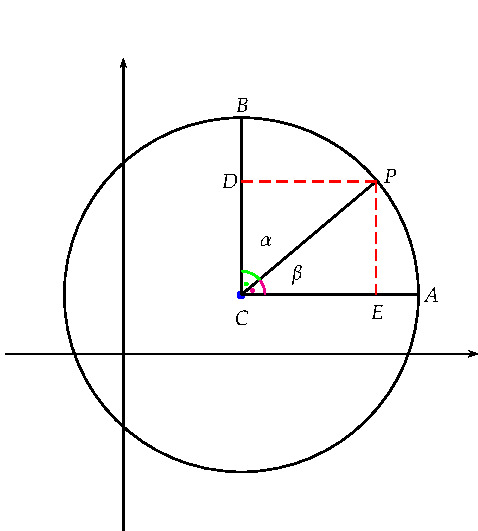
\includegraphics{circunferencia.pdf}
  % \psset{PointSymbol=none}
  % \psset{ticksize=0pt}
  % \begin{pspicture*}(-2,-3)(6,6)
  %   \psaxes[labels=none]{->}(0,0)(-1.99,-2.99)(6,5)
  %   \psdots[linecolor=blue](2,1)
  %   \pscircle(2,1){3}
  %   \pnode(2,1){A}
  %   \rput(2,0.6){$C$}
  %   \pnode(5,1){B}
  %   \rput(5.2,1){$A$}
  %   \pnode(2,4){C}
  %   \rput(2,4.2){$B$}
  %   \pnode(4.28,2.92){P}
  %   \rput(4.5,3){$P$}
  %   \rput(4.28,0.7){$E$}
  %   \rput(1.8,2.92){$D$}
  %   \psline(2,1)(5,1)
  %   \psline(2,1)(2,4)
  %   \psline(2,1)(4.28,2.92)
  %   \psline[linestyle=dashed,linecolor=red](4.28,1)(4.28,2.92)
  %   \psline[linestyle=dashed,linecolor=red](2,2.92)(4.28,2.92)
  %   \pstRightAngle[linecolor=magenta, RightAngleType=german]{B}{A}{P}
  %   \pstMarkAngle[linecolor=magenta]{B}{A}{P}{$\beta$}
  %   \pstRightAngle[linecolor=green, RightAngleType=german]{P}{A}{C}
  %   \pstMarkAngle[linecolor=green]{P}{A}{C}{$\alpha$}
  % \end{pspicture*}
\end{figure}

Na Figura \ref{circunferencia}, considere o p\'e da perpendicular ao segmento $CA$ passando por $P$ e denote esse ponto por $E$. Agora, considere o p\'e da perpendicular ao segmento $CB$ passando por $P$ e denote esse ponto por $D$. Ent\~ao os segmentos $CD$ e $EP$ t\^em o mesmo comprimento $k$. Da{\'\i}
\begin{equation}\label{equacaosenocosseno}
  \cos\alpha = \dfrac{k}{r} = \sin\beta.
\end{equation}

Substituindo \eqref{equacaosenocosseno} em \eqref{equacaoinicialY} obtemos:
\[
  \sin\beta = \dfrac{y - y_0}{r},
\]
isto \'e,
\begin{equation}\label{equacaoparametricaY}
   y = y_0 + r\sin\beta.
\end{equation}

Por outro lado, se um ponto $P(x, y)$ satisfaz as equa\c{c}\~oes \eqref{equacaoparametricaX} e \eqref{equacaoparametricaY}, ent\~ao
\[
  d(P,C) = \sqrt{(x - x_0)^2 + (y - y_0)^2} = \sqrt{r^2\cos^2\beta + r^2\sin^2\beta} = r
\]
e ent\~ao o ponto $P$ pertence \`a circunfer\^encia de centro $C(x_0,y_0)$ e raio $r$.

\begin{definicao}
  As equa\c{c}\~oes
  \[
    \begin{cases}
      x = x_0 + r\cos\beta\\
      y = y_0 + r\sin\beta,
    \end{cases}
    \beta \in [0,2\pi]
  \]
  s\~ao chamadas \textbf{equa\c{c}\~oes param\'etricas} da circunfer\^encia de centro $C(x_0, y_0)$ e raio $r$.\index{Circunfer\^encia!Equa\c{c}\~oes Param\'etricas}
\end{definicao}

Seja $C$ uma circunfer\^encia com equa\c{c}\~oes param\'etricas
\[
    \begin{cases}
      x = x_0 + r\cos\beta\\
      y = y_0 + r\sin\beta,
    \end{cases}
    \beta \in [0,2\pi].
\]

Podemos escrever
\begin{align*}
  x - x_0 = r\cos\beta\\
  y - y_0 = r\sin\beta.
\end{align*}
Elevando ao quadrado ambos os lados
\begin{align*}
  (x - x_0)^2 = r^2\cos^2\beta\\
  (y - y_0)^2 = r^2\sin^2\beta
\end{align*}
e somando obtemos
\begin{equation}
  (x - x_0)^2 + (y - y_0)^2 = r^2
\end{equation}
que \'e a \textbf{equa\c{c}\~ao cartesiana} da circunfer\^encia de centro $(x_0,y_0)$ e raio $r$.\index{Circunfer\^encia!Equa\c{c}\~ao Cartesiana}
Podemos reescrever essa equa\c{c}\~ao como
\[
  x^2 + y^2 - 2x_0x - 2y_0y + x_0^2 + y_0^2 - r^2 = 0.
\]
Fazendo
\[
  -2x_0 = a,\quad -2y_0 = b,\quad x_0^2 + y_0^2 - r^2 = c
\]
obtemos
\begin{equation}\label{equacaoalternativacircunferencia}
  x^2 + y^2 + ax + by + c = 0.
\end{equation}

Sejam $P_1(x_1,y_1)$, $P_2(x_2,y_2)$ e $P_3(x_3,y_3)$ tr\^es pontos n\~ao colineares, isto \'e, os vetores $\vec{P_1P_2}$ e $\vec{P_1P_3}$ n\~ao s\~ao paralelos. Nessa situa\c{c}\~ao \'e poss{\'\i}vel obter uma circunfer\^encia contendo estes tr\^es pontos. Para isso considere a equa\c{c}\~ao \eqref{equacaoalternativacircunferencia}. Para que $P_1$, $P_2$ e $P_3$ perten\c{c}am a uma circunfer\^encia $C$ devemos ter:
\begin{align*}
  x_1^2 + y_1^2 + ax_1 + by_1 + c = 0\\
  x_2^2 + y_2^2 + ax_2 + by_2 + c = 0\\
  x_3^2 + y_3^2 + ax_3 + by_3 + c = 0.
\end{align*}
Da{\'\i} para encontrar a circunfer\^encia desejada, basta determinar os valores de $a$, $b$ e $c$. Ou seja, precisamos resolver o sistema
\[
  \begin{cases}
    ax_1 + by_1 + c = -(x_1^2 + y_1^2)\\
    ax_2 + by_2 + c = -(x_2^2 + y_2^2)\\
    ax_3 + by_3 + c = -(x_3^2 + y_3^2).
  \end{cases}
\]

Como os ponto $P_1$, $P_2$ e $P_3$ n\~ao s\~ao colineares, este sistema sempre possui solu\c{c}\~ao \'unica.

\begin{exemplos}
  \begin{enumerate}
    \item Escreva a equa\c{c}\~ao cartesiana da circunfer\^encia passando pelos pontos $A(1,1)$, $B(1,-2)$ e $C(2,3)$.
    \begin{solucao}
      Temos
      \begin{align*}
        \vec{AB} = (0,-3)\\
        \vec{AC} = (1,2)
      \end{align*}
      assim os pontos n\~ao s\~ao colineares e portanto definem uma circunfer\^encia. Para encontr\'a-la, devemos resolver o sistema
      \[
        \begin{cases}
          a + b + c = -2\\
          a - 2b + c = -5\\
          2a + 3b + c = -13
        \end{cases}
      \]
      cuja solu\c{c}\~ao \'e
      \[
        a = -13,\quad b = 1 \quad\mbox{e}\quad c = 10.
      \]
      Logo
      \[
        x^2 + y^2 - 13x + y - 10 = 0
      \]
      \'e a equa\c{c}\~ao procurada.

      Agora, como
      \[
        -2x_0 = a,\quad -2y_0 = b,\quad x_0^2 + y_0^2 - r^2 = c
      \]
      segue que
      \[
        x_0 = 13/2,\quad y_0 = -1/2 \quad\mbox{e}\quad r^2 = 65/2.
      \]
      Assim a equa\c{c}\~ao cartesiana da circunfer\^encia ser\'a
    \[
      \left(x - \dfrac{13}{2}\right)^2 + \left(y + \dfrac{1}{2}\right)^2 = \dfrac{65}{2}.
    \]
    As equa\c{c}\~oes param\'etricas s\~ao
    \[
      \begin{cases}
        x = \dfrac{13}{2} + \dfrac{\sqrt{65}}{\sqrt{2}}\cos\beta\\
        y = -\dfrac{1}{2} + \dfrac{\sqrt{65}}{\sqrt{2}}\sin\beta\\
      \end{cases}, \beta \in [0,2\pi].
    \]
    \end{solucao}
    \item Encontre a equa\c{c}\~ao da circunfer\^encia que passa pelos pontos $P_1(1,-1)$, $P_2(0,1)$ e $P_3(1,0)$.
    \begin{solucao}
      Primeiro note que
      \begin{align*}
        \vec{P_1P_2} = (-1,2)\\
        \vec{P_1P_3} = (0,1).
      \end{align*}
      Assim os pontos n\~ao s\~ao colineares, portanto tal circunfer\^encia existe. Para encontr\'a-la, basta resolver o sistema
      \[
        \begin{cases}
          a - b + c = -2\\
          b + c = -1\\
          a + c = -2.
        \end{cases}
      \]
      A solu\c{c}\~ao \'e $a = b = 1$ e $c = -2$. Logo a circunfer\^encia tem equa\c{c}\~ao
      \[
        x^2 + y^2 + x + y - 2 = 0.
      \]
    \end{solucao}
    \item Encontre a equa\c{c}\~ao da circunfer\^encia que passa pelos pontos $P_1(1,3)$, $P_2(3,-5)$ e $P_3(2,-1)$.
    \begin{solucao}
      Note que
      \begin{align*}
        \vec{P_1P_2} = (2, -8)\\
        \vec{P_1P_3} = (1, -4).
      \end{align*}
      Assim $P_1$, $P_2$ e $P_3$ s\~ao colineares e portanto os tr\^es pontos n\~ao definem uma circunfer\^encia.
    \end{solucao}
  \end{enumerate}
\end{exemplos}

% section equacoes_da_circunferencias (end)

\section{C\^onicas} % (fold)
\label{sec:conicas}

\begin{definicao}
  Chama-se \textbf{c\^onica} o lugar geom\'etrico dos pontos $P(x,y)$ que satisfazem uma equa\c{c}\~ao do segundo grau $g(x,y) = 0$, onde\index{C\^onicas}
  \begin{equation}\label{equacaoconica}
    g(x,y) = ax^2 + bxy + cy^2 + dx + ey + f.
  \end{equation}
\end{definicao}

Na equa\c{c}\~ao \eqref{equacaoconica} pelo menos um dos n\'umeros $a$, $b$ $c$ \'e diferente de zero. Os termos $ax^2$ e $cy^2$ s\~ao os \textbf{termos quadr\'aticos}, o termo $bxy$ \'e o \textbf{termo quadr\'atico misto}, $dx$ e $ey$ s\~ao os \textbf{termos lineares} e $f$ \'e o \textbf{termo independente}. \index{C\^onica!Termos Quadr\'aticos} \index{C\^onica!Termo Quadr\'atico Misto} \index{C\^onica!Termos Lineares} \index{C\^onica!Termos Independete}

A equa\c{c}\~ao \eqref{equacaoconica} pode representar:
\begin{enumerate}[label=({\arabic*})]
  \item um conjunto vazio: $x^2 + y^2 = -1$;
  \item um conjunto formado por um ponto: $x^2 + y^2 = 0$;
  %\item uma reta;
  \item a reuni\~ao de duas retas (paralelas ou concorrentes): $x^2 - y^2 - 2x - 6y -8 =0$;
  \item uma circunfer\^encia: $x^2 + y^2 - 13x + y - 10 = 0$;
  \item uma elipse: $4x^2 + 9y^2 - 8x - 36y + 4 = 0$;
  \item uma hip\'erbole: $3x^3 + 3y^2 - 10xy + 12\sqrt{2}x - 4\sqrt{2}y + 32 = 0$;
  \item uma par\'abola: $x^2 - 2xy + y^2 -2x - 2y + 1 = 0$.
\end{enumerate}

Nos casos em que a equa\c{c}\~ao \eqref{equacaoconica} representar um conjunto vazio, um ponto, retas ou circunfer\^encias diremos que a c\^onica definida \'e uma \textbf{c\^onica degenerada}. Aqui vamos estudar as c\^onicas chamadas de elipse, hip\'erbole e par\'abola.

\subsection{Elipse} % (fold)
\label{sub:elipse}

\begin{definicao}
  Sejam $F_1$ e $F_2$ pontos distintos do plano, $2c$ a dist\^ancia entre $F_1$ e $F_2$ e $a$ um n\'umero real tal que $a > c$. O lugar geom\'etrico $\mathcal{E}$ dos pontos $P$ tais que
  \begin{equation}\label{definicaoelipse}
    d(P,F_1) + d(P,F_2) = 2a
  \end{equation}
  chama-se \textbf{elipse}. Cada um dos pontos $F_1$ e $F_2$ \'e chamado \textbf{foco} da elipse. O segmento $F_1F_2$ \'e chamado \textbf{segmento focal}, seu ponto m\'edio \'e o \textbf{centro} da elipse e $2c$ \'e chamado \textbf{dist\^ancia focal}. A reta passando por $F_1$ e $F_2$ chama-se \textbf{reta focal}.\index{Elipse} \index{Elipse!Focos} \index{Elipse!Centro} \index{Elipse!Reta Focal}
\end{definicao}

Para obter a equa\c{c}\~ao que descreve uma elipse vamos fixar os focos $F_1$ e $F_2$ como sendo $F_1(-c,0)$ e $F_2(c,0)$. Assim o centro dessa elipse estar\'a na origem do plano cartesiano. Assim, seja $P(x,y)$ um ponto pertencente \`a elipse de focos $F_1$ e $F_2$. Ent\~ao
\begin{equation}
  d(P,F_1) + d(P,F_2) = 2a,
\end{equation}
isto \'e,
\begin{equation}
  d(P,F_1) = 2a -  d(P,F_2).
\end{equation}
Assim,
\[
  \sqrt{(x + c)^2 + y^2} = 2a - \sqrt{(x - c)^2 + y^2}
\]
e elevando ao quadrado ambos os membros dessa igualdade obtemos
\[
  a\sqrt{(x - c)^2 + y^2} = a^2 - cx.
\]
Elevando novamente ao quadrado e simplificando
\[
  (a^2 - c^2)x^2 + a^2y^2 = a^2(a^2 - c^2).
\]
Fazendo $b^2 = a^2 - c^2$, podemos escrever
\[
  b^2x^2 + a^2y^2 = a^2b^2.
\]
Finalmente, dividindo por $a^2b^2$ obtemos
\begin{equation}\label{equacaoelipse}
  \elipse{a^2}{b^2}.
\end{equation}

Observe que
\begin{align}
  a^2 = b^2 + c^2\\
  a > b > 0\\
  a > c > 0.
\end{align}

Assim todo ponto pertencente a elipse de focos $F_1(-c,0)$ e $F_2(c,0)$, deve satisfazer a equa\c{c}\~ao
\[
  \elipse{a^2}{b^2}.
\]

Por outro lado, seja $Q(\alpha,\beta)$ um ponto tal que
\[
  \dfrac{\alpha^2}{a^2} + \dfrac{\beta^2}{b^2} = 1.
\]
Ent\~ao $\beta^2 = b^2 - (b^2/a^2)\alpha^2$ e da{\'\i}
\begin{align*}
  d^2(Q,F_1) &= (\alpha + c)^2 + \beta^2\\
&= \alpha^2 + 2c\alpha + c^2 + b^2 - \dfrac{b^2}{a^2}\alpha^2\\
&= \left(\dfrac{c}{a}\alpha + a\right)^2.
\end{align*}

Analogamente,
\begin{equation*}
  d^2(Q,F_2) = \left(\dfrac{c}{a}\alpha - a\right)^2.
\end{equation*}
Assim
\begin{align}
  d(Q,F_1) &= \left|\dfrac{c}{a}\alpha + a\right|\label{distanciaP1}\\
  d(Q,F_2) &= \left|\dfrac{c}{a}\alpha - a\right|\label{distanciaP2}.
\end{align}

Como
\[
  \dfrac{\alpha^2}{a^2} + \dfrac{\beta^2}{b^2} = 1.
\]
ent\~ao $\alpha^2/a^2 \le 1$, isto \'e, $\mid\alpha\mid\le a$. Mas $c/a > 0$, da{\'\i}
\[
  \dfrac{c}{a}\mid\alpha\mid \le c < a
\]
logo
\[
  -a < \dfrac{c\alpha}{a} < a.
\]
Portanto,
\begin{align*}
  \dfrac{c}{a}\alpha + a > 0\\
  \dfrac{c}{a}\alpha - a < 0.
\end{align*}
Desse modo podemos escrever \eqref{distanciaP1} e \eqref{distanciaP2} como
\begin{align*}
  d^2(Q,F_1) &= \dfrac{c}{a}\alpha + a\\
  d^2(Q,F_2) &= a - \dfrac{c}{a}\alpha.
\end{align*}

Assim
\[
  d(Q,F_1) + d(Q,F_2) = 2a
\]
e ent\~ao o ponto $Q(\alpha,\beta)$ pertence \`a elipse de focos $F_1(-c,0)$ e $F_2(c,0)$.

Os n\'umeros $a$, $b$ e $c$ s\~ao chamados \textbf{par\^ametros geom\'etricos} da elipse. A equa\c{c}\~ao \eqref{equacaoelipse} \'e chamada de \textbf{equa\c{c}\~ao reduzida da elipse} de centro $O(0,0)$ e focos no eixo $x$. Indicamos tal elipse por\index{Elipse!Par\^ametros Geom\'etricos} \index{Elipse!Equa\c{c}\~ao Reduzida}
\[
  \mathcal{E}: \elipse{a^2}{b^2}.
\]

Com isso provamos a seguinte proposi\c{c}\~ao:
\begin{proposicao}
  Um ponto $P(x,y)$ \'e um ponto da elipse de equa\c{c}\~ao reduzida
  \[
    \elipse{a^2}{b^2}
  \]
  se, e somente se, as dist\^ancias de $P$ aos focos $F_1$ e $F_2$ s\~ao
  \begin{align*}
    d^2(P,F_1) &= \dfrac{c}{a}\alpha + a\\
    d^2(P,F_2) &= a - \dfrac{c}{a}\alpha.
  \end{align*}
\end{proposicao}

\begin{observacao}
  \begin{enumerate}
    \item A equa\c{c}\~ao \eqref{equacaoelipse} s\'o \'e v\'alida para elipses com focos no eixo $x$ e centro na origem. Mudan\c{c}as nos focos ou no centro, resultar\~ao em uma equa\c{c}\~ao diferente para a elipse.
    \item Se $(x,y)$ satisfaz a equa\c{c}\~ao \eqref{equacaoelipse}, ent\~ao $(-x,-y)$, $(-x,y)$ e $(x,-y)$ tamb\'em satisfazem a mesma equa\c{c}\~ao. Assim a elipse \'e sim\'etrica em rela\c{c}\~ao ao eixo $x$, ao eixo $y$ e ao centro do plano cartesiano.
    \item O ponto $(x,0)$ pertence \`a elipse de equa\c{c}\~ao \eqref{equacaoelipse} se, e somente se, $x^2/a^2 = 1$, isto \'e, $x = \pm a$. Al\'em disso, o ponto $(0,y)$ pertence \'a elipse de equa\c{c}\~ao \eqref{equacaoelipse} se, e s\'o se, $y = \pm b$. Portanto, a interse\c{c}\~ao de $E$ com o eixo $x$ s\~ao os pontos $A_1(-a,0)$ e $A_2(a,0)$ e a interse\c{c}\~ao com o eixo $y$ s\~ao os pontos $B_1(0,-b)$ e $B_2(0,b)$. Note que $d(B_j,F_i) = \sqrt{c^2 + b^2} = a$, para $i$, $j = 1$, 2.
    \item N\~ao existe circunfer\^encia que contenha os pontos $A_1$, $A_2$, $B_1$ e $B_2$. Caso existisse, tal circunfer\^encia teria dois di\^ametros diferentes, cujos comprimento s\~ao dados pelos comprimentos dos segmente $A_1A_2$ e $B_1B_2$, o que \'e imposs{\'\i}vel. Portanto, como esses pontos pertencem a $E$, podemos afirmar que a elipse n\~ao \'e uma circunfer\^encia e nem o conjunto vazio.
  \end{enumerate}
\end{observacao}

Na equa\c{c}\~ao \eqref{equacaoelipse}, fazendo $y \ge 0$ podemos escrever
\[
  y = \dfrac{b}{a}\sqrt{a^2 - x^2},\quad x \in [0,a].
\]
Tal equa\c{c}\~ao \'e uma fun\c{c}\~ao em $x$, cont{\'\i}nua, decrescente e com concavidade para baixo em todo seu dom{\'\i}nio. Assim seu gr\'afico \'e dado pela Figura \ref{GraficoprimeiroquadranteElipse}.
\begin{figure}[h]
  \centering
  \caption{Gr\'afico da fun\c{c}\~ao $y = \dfrac{b}{a}\sqrt{a^2 - x^2}$}
  \label{GraficoprimeiroquadranteElipse}
  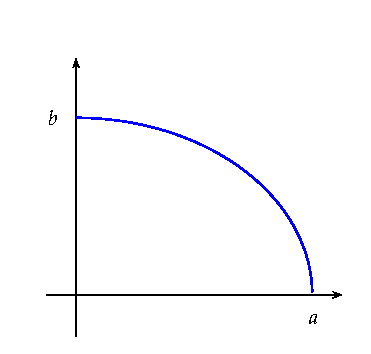
\includegraphics{grafico-elipse-primeiro-quadrante.pdf}
  % \psset{ticksize=0pt}
  % \begin{pspicture*}(-1.2,-1)(5,5)
  %   \psaxes[labels=none]{->}(0,0)(-0.5,-0.7)(4.5,4)
  %   \psplot[algebraic,linecolor=blue,plotpoints=20000]{0}{3.998888999}{(3/4)*sqrt(16 - x^2)}
  %   \rput(-0.4,3){$b$}
  %   \rput(4,-0.4){$a$}
  % \end{pspicture*}
\end{figure}

E como a elipse \'e sim\'etrica, sua forma \'e dada pela Figura \ref{FormageralElipse}.
\begin{figure}[h]
  \centering
  \caption{Elipse com focos no eixo $x$ e centro na origem: $\elipse{a^2}{b^2}$}
  \label{FormageralElipse}
  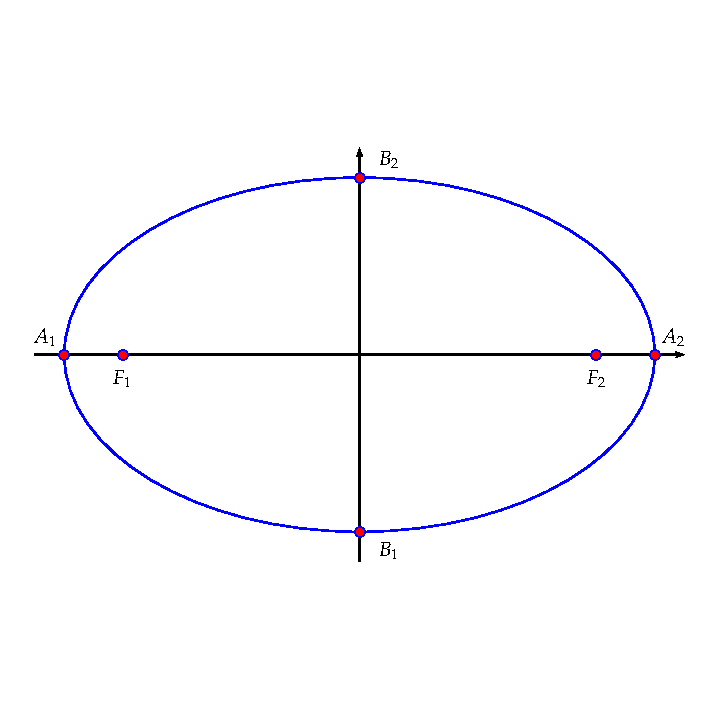
\includegraphics{elipse-focos-eixo-X.pdf}
  % \psset{ticksize=0pt}
  % \begin{pspicture*}(-7,-7)(7,7)
  %   \psaxes[labels=none]{->}(0,0)(-5.5,-3.5)(5.5,3.5)
  %   \psellipse[linecolor=blue](0,0)(5,3)
  %   \rput(5.3,0.3){$A_2$}
  %   \psdot[linecolor=blue,fillcolor=red,dotstyle=o,dotsize=5pt](5,0)
  %   \rput(-5.3,0.3){$A_1$}
  %   \psdot[linecolor=blue,fillcolor=red,dotstyle=o,dotsize=5pt](-5,0)
  %   \rput(0.5,-3.3){$B_1$}
  %   \psdot[linecolor=blue,fillcolor=red,dotstyle=o,dotsize=5pt](0,-3)
  %   \rput(0.5,3.3){$B_2$}
  %   \psdot[linecolor=blue,fillcolor=red,dotstyle=o,dotsize=5pt](0,3)
  %   \rput(4,-0.4){$F_2$}
  %   \psdot[linecolor=blue,fillcolor=red,dotstyle=o,dotsize=5pt](4,0)
  %   \rput(-4,-0.4){$F_1$}
  %   \psdot[linecolor=blue,fillcolor=red,dotstyle=o,dotsize=5pt](-4,0)
  % \end{pspicture*}
\end{figure}

\begin{definicao}
  Os pontos $A_1$ e $A_2$ em que a reta focal intercepta a elipse e os pontos $B_1$ e $B_2$ em que a mediatriz do segmento focal intercepta a elipse s\~ao chamados de \textbf{v\'ertices}. Os segmentos $A_1A_2$ e $B_1B_2$ s\~ao chamados de \textbf{eixo maior} e \textbf{eixo menor} da elipse, respectivamente.\index{Elipse!V\'ertice} \index{Elipse!Eixo Maior} \index{Elipse!Eixo Menor}
\end{definicao}

\begin{exemplos}
  \begin{enumerate}
    \item A equa\c{c}\~ao
    \[
      \elipse{9}{4}
    \]
    representa uma elipse onde $a = 3$, $b = 2$. Os focos s\~ao $F_1(-c,0)$ e $F_2(c,0)$ onde, $a^2 = b^2 + c^2$. Da{\'\i}, $a = \sqrt{5}$. Logo $F_1(-\sqrt{5},0)$ e $F_2(\sqrt{5},0)$. Os v\'ertices s\~ao $A_1(-3,0)$, $A_2(3,0)$, $B_1(0,-2)$ e $B_2(0,2)$.
    \item Encontre a equa\c{c}\~ao da elipse cujos focos s\~ao $F_1(-3,0)$ e $F_2(0,4)$ e cujo eixo maior mede 7.
    \begin{solucao}
      Como os focos n\~ao est\~ao sobre o eixo $x$, n\~ao podemos usar a equa\c{c}\~ao \eqref{equacaoelipse}. Assim vamos utilizar a defini\c{c}\~ao \eqref{definicaoelipse}. Seja $P(x,y)$ um ponto pertencente a tal elipse, ent\~ao
      \[
        d(P,F_1) + d(P,F_2) = 7.
      \]
      Assim
      \begin{align*}
        &\sqrt{(x + 3)^2 + y^2} + \sqrt{x^2 + (y - 4)^2} = 7\\
        &(x+ 3)^2 + y^2 = 49 - 14\sqrt{x^2 + (y - 4)^2} + x^2 + (y - 4)^2\\
        &(3x + 4y - 28)^2 = \left[-7\sqrt{x^2 + (y - 4)^2}\right]^2\\
        &9x^2 + 24xy + 16y^2 - 168x - 224y + 784 = 49x^2 + 49y^2 - 392y + 784
      \end{align*}
      Portanto a elipse procurada tem equa\c{c}\~ao
      \[
        40x^2 + 33y^2 - 24xy + 168x - 168y = 0.
      \]
    \end{solucao}
    \item Encontre a equa\c{c}\~ao da elipse com focos $F_1(0,-2)$ e $F_2(0,2)$ e tal que $a = 3$.
    \begin{solucao}
      Neste caso, $P(x,y)$ pertence \`a elipse se, e somente se,
      \begin{align*}
        &d(P,F_1) + d(P,F_2) = 6\\
        &\sqrt{x^2 + (y + 2)^2} + \sqrt{x^2 + (y - 2)^2} = 6\\
        &(8y - 36)^2 = \left[-12\sqrt{x^2 + (y - 2)^2}\right]^2\\
        &64y^2 - 576y + 1296 = 144x^2 + 144y^2 - 576y + 576\\
        &144x^2 + 80y^2 = 720.
      \end{align*}
      Portanto a elipse procurada tem equa\c{c}\~ao
      \[
        \elipse{5}{9}.
      \]
    \end{solucao}
  \end{enumerate}
\end{exemplos}

\begin{proposicao}
  Uma equa\c{c}\~ao da forma
  \begin{equation}\label{equacaoelipsequasegeral}
    \elipse{p}{q}
  \end{equation}
  descreve uma elipse se, e somente se, os n\'umeros reais $p$ e $q$ s\~ao distintos e positivos.
\end{proposicao}

\begin{corolario}
  Sejam $O$ a origem do plano cartesiano, $p$ e $q$ n\'umeros reais distintos e positivos. Seja $E$ a elipse de equa\c{c}\~ao \eqref{equacaoelipsequasegeral} e par\^ametros geom\'etricos $a$ e $b$.
  \begin{enumerate}
    \item Se $p > q$, ent\~ao $a^2 = p$, $b^2 = q$ e $E$ tem centro $O$ e focos no eixo $x$.
    \item Se $q > p$, ent\~ao $a^2 = q$, $b^2 = p$ e $E$ tem centro $O$ e focos no eixo $y$.
  \end{enumerate}
\end{corolario}

\begin{figure}[h]
  \centering
  \caption{Elipse com focos no eixo $y$ e centro na origem: $\elipse{a^2}{b^2}$}
  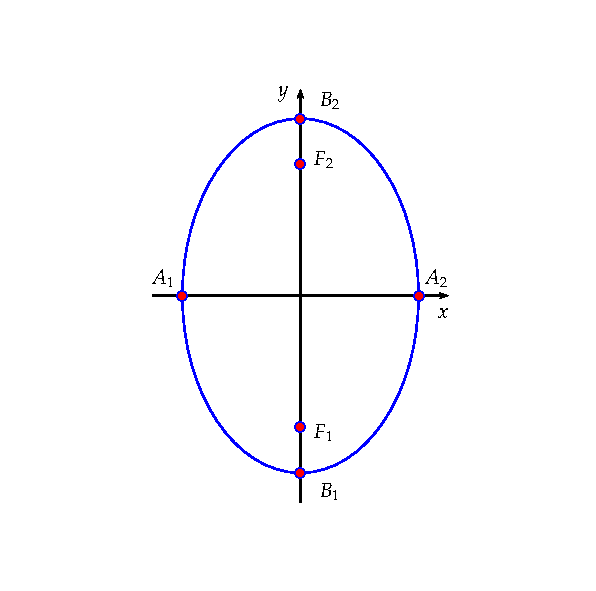
\includegraphics{elipse-focos-eixo-Y.pdf}
  % \psset{ticksize=0pt}
  % \begin{pspicture*}(-7,-7)(7,7)
  %   \psaxes[labels=none]{->}(0,0)(-2.5,-3.5)(2.5,3.5)
  %   \psellipse[linecolor=blue](0,0)(2,3)
  %   \rput(2.3,0.3){$A_2$}
  %   \psdot[linecolor=blue,fillcolor=red,dotstyle=o,dotsize=5pt](2,0)
  %   \rput(-2.3,0.3){$A_1$}
  %   \psdot[linecolor=blue,fillcolor=red,dotstyle=o,dotsize=5pt](-2,0)
  %   \rput(0.5,-3.3){$B_1$}
  %   \psdot[linecolor=blue,fillcolor=red,dotstyle=o,dotsize=5pt](0,-3)
  %   \rput(0.5,3.3){$B_2$}
  %   \psdot[linecolor=blue,fillcolor=red,dotstyle=o,dotsize=5pt](0,3)
  %   \rput(0.4,2.3){$F_2$}
  %   \psdot[linecolor=blue,fillcolor=red,dotstyle=o,dotsize=5pt](0,2.23)
  %   \rput(0.4,-2.3){$F_1$}
  %   \psdot[linecolor=blue,fillcolor=red,dotstyle=o,dotsize=5pt](0,-2.23)
  %   \rput(2.4,-0.3){$x$}
  %   \rput(-0.3,3.4){$y$}
  % \end{pspicture*}
\end{figure}


\begin{exemplos}
  Para as equa\c{c}\~oes dadas, encontre os focos, v\'ertices e o comprimento do eixo maior e menor da elipse dada.
  \begin{enumerate}
    \item $16x^2 + y^2 = 1$
    \begin{solucao}
      Podemos escrever essa equa\c{c}\~ao como
      \[
        \elipse{\dfrac{1}{16}}{1}
      \]
      e da{\'\i} $p = 1/16$ e $q = 1$. Como $p < q$, os focos est\~ao no eixo $y$. Assim $a = 1$ e $b = 1/4$. Como $a^2 = b^2 + c^2$, temos $c = \sqrt{15}/4$. Logos
      \begin{align*}
        F_1\left(0,-\dfrac{\sqrt{15}}{4}\right),\quad F_2\left(0,\dfrac{\sqrt{15}}{4}\right)\\
        A_1(0,-1),\quad A_2(0,1)\\
        B_1\left(-\dfrac{1}{4},0\right),\quad B_1\left(\dfrac{1}{4},0\right).
      \end{align*}
    \end{solucao}
    \item $25x^2 + 169y^2 = 9$
    \begin{solucao}
      Podemos escrever essa equa\c{c}\~ao como
      \[
        \elipse{\dfrac{9}{25}}{\dfrac{9}{169}}
      \]
      e da{\'\i} $p = 9/25$ e $q = 9/169$. Como $p > q$, os focos est\~ao no eixo $x$. Assim $a = 3/5$ e $b = 3/13$. Como $a^2 = b^2 + c^2$, temos $c = 36/65$. Logos
      \begin{align*}
        F_1\left(-\dfrac{36}{65}\right),\quad F_2\left(\dfrac{36}{65}\right)\\
        A_1\left(-\dfrac{3}{5},0\right),\quad A_2\left(\dfrac{3}{5},0\right)\\
        B_1\left(0,-\dfrac{3}{13}\right),\quad B_1\left(0,\dfrac{3}{13}\right).
      \end{align*}
    \end{solucao}
  \end{enumerate}
\end{exemplos}

Considere a elipse de equa\c{c}\~ao reduzida
\[
  \mathcal{E}: \elipse{a^2}{b^2},\quad a > b.
\]
Temos
\begin{align*}
  \dfrac{x^2}{a^2} \le 1 \Leftrightarrow -a \le x \le a\\
  \dfrac{y^2}{b^2} \le 1 \Leftrightarrow -b \le x \le b.
\end{align*}
Portanto os pontos de $\mathcal{E}$ est\~ao dentro do ret\^angulo
\begin{figure}[!h]
  \centering
  \caption{Ret\^angulo fundamental}
  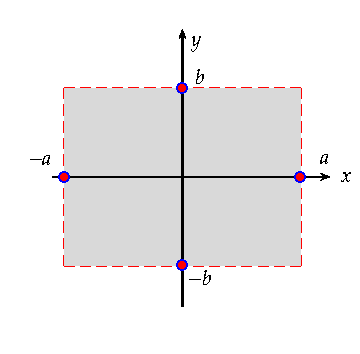
\includegraphics{retangulo-fundamental.pdf}
  % \psset{ticksize=0pt}
  % \begin{pspicture*}(-3,-3)(3,3)
  %   \psline[linestyle=dashed,linecolor=red](2,-1.5)(2,1.5)
  %   \psline[linestyle=dashed,linecolor=red](-2,-1.5)(-2,1.5)
  %   \psline[linestyle=dashed,linecolor=red](-2,1.5)(2,1.5)
  %   \psline[linestyle=dashed,linecolor=red](-2,-1.5)(2,-1.5)
  %   \pscustom[fillstyle=solid,fillcolor=gray!30,linestyle=none]
  %   {
  %     \psline(2,-1.5)(2,1.5)
  %     \psline(-2,-1.5)(-2,1.5)
  %     \psline(-2,1.5)(2,1.5)
  %     \psline(-2,-1.5)(2,-1.5)
  %   }
  %   \psaxes[labels=none]{->}(0,0)(-2.2,-2.2)(2.5,2.5)[$x$,0][$y$,-45]
  %   \psdot[linecolor=blue,fillcolor=red,dotstyle=o,dotsize=5pt](2,0)
  %   \rput(2.4,0.3){$a$}
  %   \psdot[linecolor=blue,fillcolor=red,dotstyle=o,dotsize=5pt](-2,0)
  %   \rput(-2.4,0.3){$-a$}
  %   \psdot[linecolor=blue,fillcolor=red,dotstyle=o,dotsize=5pt](0,1.5)
  %   \rput(0.3,1.7){$b$}
  %   \psdot[linecolor=blue,fillcolor=red,dotstyle=o,dotsize=5pt](0,-1.5)
  %   \rput(0.3,-1.7){$-b$}
  % \end{pspicture*}
\end{figure}
Esse ret\^angulo \'e chamado de \textbf{ret\^angulo fundamental} da elipse $\mathcal{E}$.\index{Elipse!Ret\^angulo Fundamental}

Agora, como $a > b$, ent\~ao
\[
  \dfrac{x^2}{a^2} + \dfrac{y^2}{a^2} \le \dfrac{x^2}{a^2} + \dfrac{y^2}{b^2} \le \dfrac{x^2}{b^2} + \dfrac{y^2}{b^2}.
\]
Assim, todo ponto $P(x,y)$ de $E$ satisfaz
\[
  \dfrac{x^2}{a^2} + \dfrac{y^2}{a^2} \le 1 \le \dfrac{x^2}{b^2} + \dfrac{y^2}{b^2}.
\]
e da{\'\i} $b^2 \le x^2 + y^2 \le a^2$, ou seja, $b \le d(P,O) \le a$. Portanto a elipse est\'a contida entre as circunfer\^encias de raio $a$ e $b$. Essa regi\~ao \'e chamada de \textbf{coroa fundamental} da elipse.\index{Elipse!Coroa Fundamental}
\begin{figure}[!h]
  \centering
  \caption{Coroa Fundamental}
  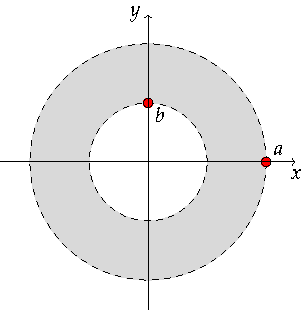
\includegraphics{coroa-fundamental.pdf}
  % \begin{tikzpicture}
  %   \coordinate (F) at (-2.5,0);
  %   \coordinate (G) at (0,-2.5);
  %   \coordinate (X) at (2.5,0);
  %   \coordinate (Y) at (0,2.5);
  %   \coordinate[label=right:$a$] (A) at (2,0.2);
  %   \coordinate[label=right:$b$] (B) at (0,0.8);
  %   % Styles
  %   \tikzstyle{axes}=[]

  %   \draw[fill=gray!30,even odd rule,style=dashed] (0,0) circle (2cm) circle (1cm) ;
  %   \draw[fill=red] (0,1) circle (0.08cm);
  %   \draw[fill=red] (2,0) circle (0.08cm);
  %   \begin{scope}[style=axes]%constr\'oi os eixos cartesianos
  %     \draw[->] (F) -- (X) node[below] {$x$} coordinate(x axis);
  %     \draw[->] (G) -- (Y) node[left] {$y$} coordinate(y axis);
  %   \end{scope}
  % \end{tikzpicture}
\end{figure}

Logo os pontos da elipse est\~ao na regi\~ao compreendida entre o ret\^angulo fundamental e a coroa fundamental.
\begin{figure}[!h]
  \centering
  \caption{Regi\~ao onde se encontram os pontos de uma elipse}
  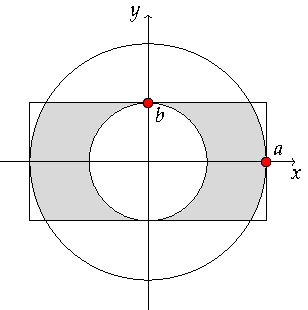
\includegraphics{regiao-fundamental.pdf}
  % \begin{tikzpicture}
  %   \coordinate (F) at (-2.5,0);
  %   \coordinate (G) at (0,-2.5);
  %   \coordinate (X) at (2.5,0);
  %   \coordinate (Y) at (0,2.5);
  %   \coordinate[label=right:$a$] (A) at (2,0.2);

  %   \begin{scope}
  %     \clip (-2,-1) rectangle (2,1);
  %     \fill[gray!30] (0,0) circle (2cm);
  %     \fill[white] (0,0) circle (1cm);
  %   \end{scope}

  %   \draw[name path=rf](-2,-1) rectangle (2,1);
  %   \draw[name path=cf2] (0,0) circle (2);
  %   \draw[name path=cf1] (0,0) circle (1cm);
  %   \coordinate[label=right:$b$] (B) at (0,0.8);
  %   \tikzstyle{axes}=[]
  %   \begin{scope}[style=axes]%constr\'oi os eixos cartesianos
  %     \draw[->] (F) -- (X) node[below] {$x$} coordinate(x axis);
  %     \draw[->] (G) -- (Y) node[left] {$y$} coordinate(y axis);
  %   \end{scope}
  %   \draw[fill=red] (0,1) circle (0.08cm);
  %   \draw[fill=red] (2,0) circle (0.08cm);
  % \end{tikzpicture}
\end{figure}
Assim observe que se $b/a$ estiver pr\'oximo de 1, ent\~ao o ret\^angulo fundamental ser\'a pr\'oximo de um quadrado e da{\'\i} a forma da elipse se aproximar\'a de um circunfer\^encia. Por outro lado, quanto mais pr\'oximo de 0 estiver $b/a$, mas alongada ser\'a a elipse. Mas, sabemos que
\[
  a^2 = b^2 + c^2
\]
da{\'\i}
\[
  \left(\dfrac{b}{a}\right)^2 + \left(\dfrac{c}{a}\right)^2 = 1.
\]
Dessa equa\c{c}\~ao vemos que se $b/a \to 1$, ent\~ao $c/a \to 0$ e da{\'\i} os focos de $\mathcal{E}$ est\~ao ``mais pr\'oximos'' de seu centro do que de seus v\'ertices e desse modo a elipse ser\'a mais parecida com um circunfer\^encia. Por outro lado, se $b/a \to 0$, ent\~ao $c/a \to 1$ e assim os focos de $\mathcal{E}$ est\~ao ``mais pr\'oximos'' dos v\'ertices do que do centro de $\mathcal{E}$ e desse modo a elipse ser\'a mais alongada.  Portanto o quociente $c/a$ mede o quanto os focos de $\mathcal{E}$ est\~ao ``fora do centro''. A essa raz\~ao damos o nome de \textbf{excentricidade} (\textit{ex centrum}) da elipse e representamos por\index{Elipse!Excentricidade}
\[
  e = \dfrac{c}{a}.
\]

% subsection elipse (end)

\subsection{Hip\'erbole} % (fold)
\label{sub:hiperbole}

\begin{definicao}
  Sejam $F_1$ e $F_2$ pontos distintos do plano tais que sua dist\^ancia seja $2c$. Considere um n\'umero real $a$ tal que $0 < a < c$. O lugar geom\'etrico $\mathcal{H}$ dos pontos $P(x,y)$ tais que 
  \begin{equation}\label{equacaohiperbole}
    | d(P,F) - d(P,F_2)| = 2a
  \end{equation}
  chama-se \textbf{hip\'erbole}. Os pontos $F_1$ e $F_2$ s\~ao chamados \textbf{focos} da hip\'erbole, o segmento $F_1F_2$ \'e chamado \textbf{segmento focal}, o ponto m\'edio do segmento $F_1F_2$ \'e chamada de \textbf{centro} da hip\'erbole e o n\'umero $2c$ \'e chamado de \textbf{dist\^ancia focal}. A reta passando por $F_1$ e $F_2$ \'e chamada \textbf{reta focal}.\index{Hip\'erbole} \index{Hip\'erbole!Focos} \index{Hip\'erbole!Segmento Focal} \index{Hip\'erbole!Centro} \index{Hip\'erbole!Dist\^ancia Focal} \index{Hip\'erbole!Reta Focal}
\end{definicao}

Vamos fixar $F_1(-c,0)$ e $F_2(c,0)$. Assim um ponto $P(x,y)$ pertence \`a hip\'erbole $\mathcal{H}$ de focos $F_1$ e $F_2$ se
\begin{align*}
  &| d(P,F_1) - d(P,F_2) | = 2a\\
  &d(P,F_1) - d(P,F_2) = \pm 2a\\
  &d(P,F_1) = \pm 2a + d(P,F_2)\\
  &\left[\sqrt{(x + c)^2 + y^2}\right]^2 = \left[\pm 2a + \sqrt{(x - c)^2 + y^2}\right]^2\\
  &(cx - a^2)^2 = \left[\pm a\sqrt{(x - c)^2 + y^2}\right]^2\\
  &(c^2 - a^2)x^2 - a^2y^2 = a^2(c^2 - a^2).
\end{align*}
Fazendo $b^2 = c^2 - a^2$ e dividindo por $a^2b^2$ obtemos
\begin{equation}
  \dfrac{x^2}{a^2} - \dfrac{y^2}{b^2} = 1
\end{equation}
Como no caso da elipse, tamb\'em temos as rela\c{c}\~oes
\begin{align}
  c^2 = a^2 + b^2\\
  c > b > 0\label{pitagorashiperbole}\\
  c > a > 0.
\end{align}
Portanto, se um ponto $P(x,y)$ pertence \`a hip\'erbole $\mathcal{H}$, ent\~ao ele satisfaz a equa\c{c}\~ao \eqref{equacaohiperbole}.

Agora, dado um ponto $A(\alpha,\beta)$ que satisfaz a equa\c{c}\~ao \eqref{equacaohiperbole}, queremos mostrar que $A$ pertence \`a hip\'erbole $\mathcal{H}$. Temos
\begin{align}
  \dfrac{\alpha^2}{a^2} - \dfrac{\beta^2}{b^2} = 1\nonumber\\
  \beta^2 = \dfrac{b^2}{a^2}\alpha^2 - b^2.\label{equacaoauxiliarhiperbole}
\end{align}
Usando \eqref{pitagorashiperbole} e \eqref{equacaoauxiliarhiperbole}:
\begin{align*}
  d^2(P,F_1) &= (\alpha + c)^2 + \beta^2\\
  &= \alpha^2 + 2\alpha c + cˆ2 + \dfrac{b^2}{a^2}\alpha^2 - b^2
\end{align*}
donde
\[
  d^2(A,F_1) = \left(\dfrac{c}{a}\alpha + a\right)^2.
\]
Do mesmo modo, obtemos
\[
  d^2(A,F_2) = \left(\dfrac{c}{a}\alpha - a\right)^2.
\]
Assim
\begin{align}
  d(A,F_1) = \left|\dfrac{c}{a}\alpha + a\right|\\
  d(A,F_2) = \left|\dfrac{c}{a}\alpha - a\right|.
\end{align}

Mas
\[
  \dfrac{\alpha^2}{a^2} - \dfrac{\beta^2}{b^2} = 1
\]
assim 
\begin{equation}\label{pontohiperbole}
  \alpha^2/a^2 \ge 1,
\end{equation}
isto \'e, $\alpha \le -a$ ou $\alpha \ge a$. Temos ent\~ao dois casos para analisar:
\begin{enumerate}
  \item Se $\alpha \le -a$, ent\~ao
  \[
    \dfrac{c}{a}\alpha \le -c < -a.
  \]
  Portanto, $(c/a)\alpha + a < 0$ e $(c/a)\alpha - a < 0$, donde
  \begin{align*}
  d(A,F_1) = -\dfrac{c}{a}\alpha - a\\
  d(A,F_2) = -\dfrac{c}{a}\alpha + a.
\end{align*}
e ent\~ao
\[
  | d(P,F_1) - d(P,F_2)| = |-2a| = 2a.
\]
\item Se $\alpha \ge -a$, ent\~ao
  \[
    \dfrac{c}{a}\alpha \le c > a.
  \]
  Portanto, $(c/a)\alpha + a > 0$ e $(c/a)\alpha - a > 0$, donde
  \begin{align*}
  d(A,F_1) = \dfrac{c}{a}\alpha + a\\
  d(A,F_2) = \dfrac{c}{a}\alpha - a.
\end{align*}
e ent\~ao
\[
  | d(P,F_1) - d(P,F_2)| = |2a| = 2a.
\]
\end{enumerate}
Portanto, se $A(\alpha,\beta)$ satisfaz a equa\c{c}\~ao \eqref{equacaohiperbole}, ent\~ao $A$ pertence \`a hip\'erbole de focos $F_1(-c,0)$ e $F_2(c,0)$. Assim provamos a seguinte proposi\c{c}\~ao:

\begin{proposicao}
  Um ponto $P(x, y)$ \'e um ponto da hip\'erbole
  \[
    \mathcal{H}:\ \dfrac{x^2}{a^2} - \dfrac{y^2}{b^2} = 1
  \]
  se, e somente se, as dist\^ancias de $P$ aos focos s\~ao:
  \begin{align*}
    d(A,F_1) = \left|\dfrac{c}{a}\alpha + a\right|\\
    d(A,F_2) = \left|\dfrac{c}{a}\alpha - a\right|.
  \end{align*}
\end{proposicao}

Os n\'umeros $a$, $b$ e $c$ s\~ao chamados \textbf{par\^ametros geom\'etricos} da hip\'erbole $\mathcal{H}$ e a equa\c{c}\~ao
\[
  \dfrac{x^2}{a^2} - \dfrac{y^2}{b^2} = 1
\]
\'e chamada de \textbf{equa\c{c}\~ao reduzida} da hip\'erbole.\index{Hip\'erbole!Par\^ametros Geom\'etricos} \index{Hip\'erbole!Equa\c{c}\~ao Reduzida}

\begin{observacao}
  Seja $\mathcal{H} : \dfrac{x^2}{a^2} - \dfrac{y^2}{b^2} = 1$ uma hip\'erbole de focos no eixo $x$.
  \begin{enumerate}
    \item Nenhum ponto $P(x,y)$ de $\mathcal{H}$ \'e tal que $-a < x < a$, pois caso contr\'ario ter{\'\i}amos $x^2 < a^2$ o que contradiz a inequa\c{c}\~ao \eqref{pontohiperbole}. Para a ordenada $y$ n\~ao h\'a restri\c{c}\~ao, isto \'e, qualquer que seja $y$ existe $x$ tal que $\dfrac{x^2}{a^2} - \dfrac{y^2}{b^2} = 1$. Assim a hip\'erbole n\~ao \'e limitada.
    \item Se $(x,y)$ pertence a $H$, ent\~ao $(-x,-y)$, $(x,-y)$ e $(-x,y)$ tamb\'em pertencem a $\mathcal{H}$. Logo a hip\'erbole \'e sim\'etrica em rela\c{c}\~ao ao eixo $x$, ao eixo $y$  e em rela\c{c}\~ao \`a origem do plano cartesiano.
    \item O ponto $(x,0)$ pertence \`a hip\'erbole $\mathcal{H}$ se, e s\'o se, $x = \pm a$. Por isso a interse\c{c}\~ao de $\mathcal{H}$ com a reta focal s\~ao os pontos $A_1(-a,0)$ e $A_2(a,0)$, chamados de \textbf{v\'ertices} de $\mathcal{H}$.\index{Hip\'erbole!V\'ertices}
  \end{enumerate}
\end{observacao}

Considere a hip\'erbole $\mathcal{H}$ de equa\c{c}\~ao reduzida
\[
  \mathcal{H} : \dfrac{x^2}{a^2} - \dfrac{y^2}{b^2} = 1
\]
com focos $F_1(-c,0)$ e $F_2(c,0)$. Dada uma reta $r$ de equa\c{c}\~ao $y = mx$, quais as condi\c{c}\~oes sobre $a$, $b$, $c$ e $m$ para que a reta $r$ intercepte $\mathcal{H}$?

Seja $P(x_0,y_0)$ um ponto de interse\c{c}\~ao entre $r$ e $\mathcal{H}$. Ent\~ao temos
\begin{align*}
  \dfrac{x_0^2}{a^2} - \dfrac{y_0^2}{b^2} = 1\\
  y_0 = mx_0,
\end{align*}
isto \'e,
\[
  \dfrac{x_0^2}{a^2} - \dfrac{m^2x_0^2}{b^2} = 1.
\]
Resolvendo em $x_0$ obtemos
\begin{equation}\label{intersecaohiperbolereta}
x_0 = \pm \dfrac{ab}{\sqrt{b^2 - a^2m^2}} = \pm \dfrac{b}{\sqrt{\dfrac{b^2}{a^2} - m^2}}.
\end{equation}
Assim
\[
  b^2 - a^2m^2 > 0 \Leftrightarrow m^2 < \dfrac{b^2}{a^2}.
\]
Como $a$ e $b$ s\~ao positivos
\[
  -\dfrac{b}{a} < m < \dfrac{b}{a}.
\]
Logo a reta $y = mx$ intercepta a hip\'erbole $\mathcal{H}$ se, e s\'o se, seu coeficiente angular est\'a entre $-b/a$ e $b/a$. Portanto as retas
\[
  y = -\dfrac{b}{a}x \quad \mbox{e}\quad y = \dfrac{b}{a}x
\]
n\~ao interceptam a hip\'erbole $\mathcal{H}$. Tais retas s\~ao chamadas de \textbf{ass{\'\i}ntotas da hip\'erbole}. Mais ainda, da equa\c{c}\~ao \eqref{intersecaohiperbolereta} quando $m \to b/a$, o ponto $x_0$ tende para mais ou menos infinito. Logo os pontos da hip\'erbole se aproximam das ass{\'\i}ntotas a medida que $x$ se afasta da origem.\index{Hip\'erbole!Ass{\'\i}ntotas}

Como no caso da elipse, utilizando a simetria e as ass{\'\i}ntodas da hip\'erbole, podemos mostrar a partir da equa\c{c}\~ao
\[
  y = \dfrac{b}{a}\sqrt{x^2 - a^2}, \quad x \ge a
\]
que a forma da hip\'erbole ser\'a dada pela Figura \ref{FormageralHiperbole}.
\begin{figure}[!h]
  \centering
  \caption{Hip\'erbole $\dfrac{x^2}{a^2} - \dfrac{y^2}{b^2} = 1$  com ass{\'\i}ntotas $y = -\dfrac{b}{a}x$ e $y = \dfrac{b}{a}x$}
  \label{FormageralHiperbole}
  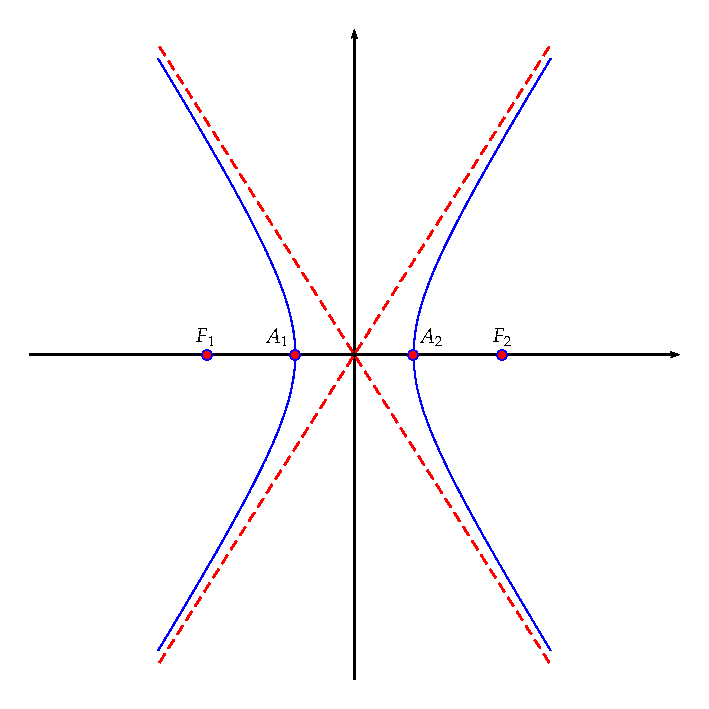
\includegraphics{hiperbole-focos-eixo-X.pdf}
  % \psset{ticksize=0pt}
  % \begin{pspicture*}(-6,-6)(6,6)
  %   \psaxes[labels=none]{->}(0,0)(-5.5,-5.5)(5.5,5.5)
  %   \psplot[algebraic,linestyle=dashed,linecolor=red]{-3.3}{3.3}{-1.58*x}
  %   \psplot[algebraic,linestyle=dashed,linecolor=red]{-3.3}{3.3}{1.58*x}
  %   \psplotImp[algebraic,linecolor=blue,stepFactor=0.1,linewidth=0.5pt](-5,-5)(5,5){x^2-y^2/2.5-1}
  %   \rput(1.3,0.3){$A_2$}
  %   \rput(-1.3,0.3){$A_1$}
  %   \rput(2.5,0.3){$F_2$}
  %   \rput(-2.5,0.3){$F_1$}
  %   \psdot[linecolor=blue,fillcolor=red,dotstyle=o,dotsize=5pt](-1,0)
  %   \psdot[linecolor=blue,fillcolor=red,dotstyle=o,dotsize=5pt](1,0)
  %   \psdot[linecolor=blue,fillcolor=red,dotstyle=o,dotsize=5pt](-2.5,0)
  %   \psdot[linecolor=blue,fillcolor=red,dotstyle=o,dotsize=5pt](2.5,0)
  % \end{pspicture*}
\end{figure}

\begin{exemplos}
  \begin{enumerate}
    \item Encontre a equa\c{c}\~ao da hip\'erbole cujos v\'ertices s\~ao $(-15,0)$ e $(15,0)$ e as ass{\'\i}ntotas t\^em equa\c{c}\~oes $5y - 4x = 0$ e $5y + 4x = 0$.
    \begin{solucao}
      As ass{\'\i}ntotas s\~ao dadas por
      \[
        y = -\dfrac{b}{a}x \quad\mbox{e }\quad y = \dfrac{b}{a}x.
      \]
      A partir dos v\'ertices encontramos $a = 15$. Da{\'\i} $b = 12$ e ent\~ao a equa\c{c}\~ao da hip\'erbole \'e
      \[
        \dfrac{x^2}{225} - \dfrac{y^2}{144} = 1.
      \]
    \end{solucao}
    \item Encontre a equa\c{c}\~ao da hip\'erbole de focos $F_1(0,-\sqrt{20})$ e $F_1(0,\sqrt{20})$ e tal que $a = 2$.
    \begin{solucao}
      Como os focos n\~ao est\~ao no eixo $x$, vamos usar a equa\c{c}\~ao \eqref{equacaohiperbole}:
      \begin{align*}
        &\mid d(P,F) - d(P,F_2)\mid = 4\\
        &\left[\sqrt{x^2 + (y + \sqrt{20})^2}\right]^2 = \left[\pm 4 + \sqrt{x^2 + (y - \sqrt{20})^2}\right]^2\\
        &(y\sqrt{20} - 4)^2 = \left[\pm 2\sqrt{x^2 + (y - \sqrt{20})^2}\right]^2\\
        &20y^2 - 8\sqrt{20}y + 16 = 4x^2 + 4y^2 - 8\sqrt{20}y + 80\\
        &16y^2 - 4x^2 = 64.
      \end{align*}
      Logo a hip\'erbole procurada tem equa\c{c}\~ao
      \[
        \dfrac{y^2}{4} - \dfrac{x^2}{16} = 1.
      \]
      Portanto as ass{\'\i}ntotas s\~ao
      \[
        y = -2x \quad\mbox{e }\quad y = 2x.
      \]
    \end{solucao}
  \end{enumerate}
\end{exemplos}

\begin{proposicao}
  Um equa\c{c}\~ao da forma
  \begin{equation}\label{hiperbolegeral}
    \dfrac{x^2}{p} + \dfrac{y^2}{q} = 1
  \end{equation}
  descreve uma hip\'erbole se, e somente se, os n\'umeros reais $p$ e $q$ s\~ao de sinal contr\'ario.
\end{proposicao}

\begin{corolario}
  Sejam $p$ e $q$ n\'umeros reais de sinal contr\'ario e $\mathcal{H}$ a hip\'erbole de equa\c{c}\~ao \eqref{hiperbolegeral} e par\^ametros geom\'etricos $a$ e $b$.
  \begin{enumerate}
    \item Se $p > 0$ e $q < 0$, ent\~ao $a^2 = p$ e $b^2 = -q$, $\mathcal{H}$ tem centro na origem e focos no eixo $x$.
    \item Se $p < 0$ e $q > 0$, ent\~ao $a^2 = q$ e $b^2 = -p$, $\mathcal{H}$ tem centro na origem e focos no eixo $y$.
  \end{enumerate}
\end{corolario}

\begin{observacao}
  No caso de uma hip\'erbole $\mathcal{H}$ com focos no eixo $y$, isto \'e, com equa\c{c}\~ao
  \[
    \mathcal{H}: \dfrac{y^2}{a^2} - \dfrac{x^2}{b^2} = 1
  \]
  as ass{\'\i}ntotas ter\~ao equa\c{c}\~oes dadas por
  \[
    x = \pm \dfrac{a}{b}y.
  \]
\end{observacao}

\begin{figure}[h]
  \centering
  \caption{Hip\'erbole $\dfrac{y^2}{b^2} - \dfrac{x^2}{a^2} = 1$ com ass{\'\i}ntotas $x = -\dfrac{a}{b}y$ e $x = \dfrac{a}{b}y$}
  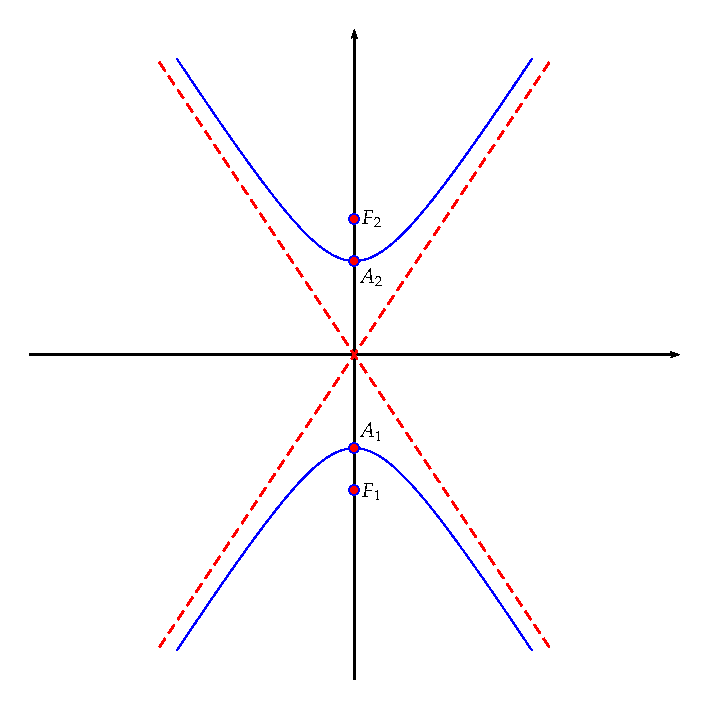
\includegraphics{hiperbole-focos-eixo-Y.pdf}
  % \psset{ticksize=0pt}
  % \begin{pspicture*}(-6,-6)(6,6)
  %   \psaxes[labels=none]{->}(0,0)(-5.5,-5.5)(5.5,5.5)
  %   \psplot[algebraic,linestyle=dashed,linecolor=red]{-3.3}{3.3}{-1.5*x}
  %   \psplot[algebraic,linestyle=dashed,linecolor=red]{-3.3}{3.3}{1.5*x}
  %   \psplotImp[algebraic,linecolor=blue,stepFactor=0.1,linewidth=0.5pt](-5,-5)(5,5){y^2/2.5 - x^2-1}
  %   \rput(0.3,1.3){$A_2$}
  %   \rput(0.3,-1.3){$A_1$}
  %   \rput(0.3,2.3){$F_2$}
  %   \rput(0.3,-2.3){$F_1$}
  %   \psdot[linecolor=blue,fillcolor=red,dotstyle=o,dotsize=5pt](0,-1.58)
  %   \psdot[linecolor=blue,fillcolor=red,dotstyle=o,dotsize=5pt](0,1.58)
  %   \psdot[linecolor=blue,fillcolor=red,dotstyle=o,dotsize=5pt](0,-2.3)
  %   \psdot[linecolor=blue,fillcolor=red,dotstyle=o,dotsize=5pt](0,2.3)
  % \end{pspicture*}
\end{figure}

% subsection hiperbole (end)



\subsection{Par\'abola} % (fold)
\label{sub:parabolas}

\begin{definicao}
  Seja $r$ uma reta e $F$ um ponto que n\~ao pertence a $r$. O lugar geom\'etrico $\mathcal{P}$ dos pontos equidistantes de $F$ e $r$ chama-se \textbf{par\'abola}. O ponto $F$ \'e chamado de \textbf{foco da par\'abola} e $r$ de \textbf{reta diretriz}.\index{Par\'abola} \index{Par\'abola!Focos} A reta contendo o foco $F$ e perpendicular \`a reta diretriz \'e chamada de \textbf{reta focal}.\index{Par\'abola!Reta diretriz}\index{Par\'abola!Reta focal}
\end{definicao}


Vamos fixar $F(p,0)$ e $r: x = -p$, onde $p > 0$. Assim um ponto $A(x,y)$ pertence \`a par\'abola de foco $F$ e reta diretriz $r$ se, e somente se,
\begin{figure}[!h]%par\'abola
  \centering
  \caption{Defini\c{c}\~ao da Par\'abola}
  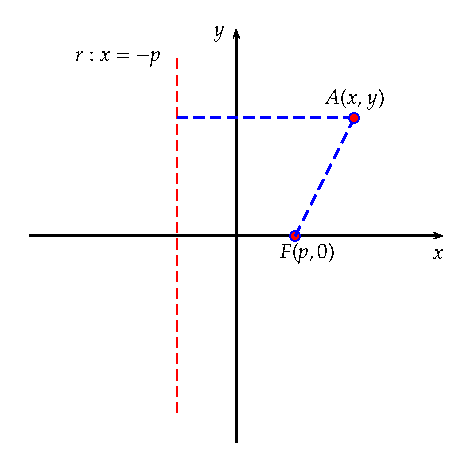
\includegraphics{parabola.pdf}
  % \psset{ticksize=0pt}
  % \begin{pspicture*}(-4,-4)(4,4)
  %   \psaxes[labels=none]{->}(0,0)(-3.5,-3.5)(3.5,3.5)
  %   \psline[linestyle=dashed,linecolor=red](-1,-3)(-1,3)
  %   \rput(1.2,-0.3){$F(p,0)$}
  %   \psdot[linecolor=blue,fillcolor=red,dotstyle=o,dotsize=5pt](1,0)
  %   \rput(2,2.3){$A(x,y)$}
  %   \psline[linestyle=dashed,linecolor=blue](1,0)(2,2)
  %   \psline[linestyle=dashed,linecolor=blue](-1,2)(2,2)
  %   \psdot[linecolor=blue,fillcolor=red,dotstyle=o,dotsize=5pt](2,2)
  %   \rput(-2,3){$r: x = -p$}
  %   \rput(3.4,-0.3){$x$}
  %   \rput(-0.3,3.4){$y$}
  % \end{pspicture*}
\end{figure}

\[
  d(A,r) = d(A,F).
\]
Mas
\begin{align*}
  d(A,r) = |x + p|\\
  d(A,F) = \sqrt{(x - p)^2 + y^2}.
\end{align*}
Logo $A$ pertence \`a par\'abola $\mathcal{P}$ se, e somente se,
\begin{align*}
  (|x + p|)^2 = (x - p)^2 + y^2\\
  x^2 + 2px + p^2 = x^2 - 2px + p^2 + y^2.
\end{align*}
Portanto $A(x,y)$ pertence \`a par\'abola $\mathcal{P}$ se, e somente se,
\begin{equation}\label{equacaoparabola}
  y^2 = 4px
\end{equation}

A equa\c{c}\~ao \eqref{equacaoparabola} \'e chamada de \textbf{equa\c{c}\~ao reduzida} da par\'abola $\mathcal{P}$. Indica-se\index{Par\'abola!Equa\c{c}\~ao reduzida}
\[
  \mathcal{P}:\ y^2 = 4px.
\]

\begin{observacao}
  \begin{enumerate}
    \item Se $(x,y)$ satisfaz a equa\c{c}\~ao \eqref{equacaoparabola}, ent\~ao $x \ge 0$, isto \'e, nenhum ponto de $\mathcal{P}$ tem abscissa negativa. J\'a para a ordenada $y$, n\~ao existem restri\c{c}\~oes. Logo a par\'abola n\~ao \'e limitada.
    \item Se $(x,y)$ pertence a $\mathcal{P}$, ent\~ao $(x,-y)$ tamb\'em pertence a $\mathcal{P}$. Logo a par\'abola \'e sim\'etrica em rela\c{c}\~ao ao eixo $x$.
    \item O \'unico ponto de interse\c{c}\~ao de $\mathcal{P}$ com os eixos coordenados \'e o ponto $(0,0)$. Tal ponto \'e chamado de \textbf{v\'ertice} da par\'abola.\index{Par\'abola!V\'ertice}
  \end{enumerate}
\end{observacao}

Na equa\c{c}\~ao \eqref{equacaoparabola} podemos isolar $x$ e escrever
\[
  x = \dfrac{y^2}{4p}
\]
obtendo assim $x$ como uma fun\c{c}\~ao de $y$. Logo o gr\'afico da par\'abola $\mathcal{P}$ \'e:

\begin{figure}[!h]%par\'abola
  \centering
  \caption{Par\'abola $\mathcal{P}: y^2 = 4px$ e reta diretriz $r: x = -p$, $p > 0$}
  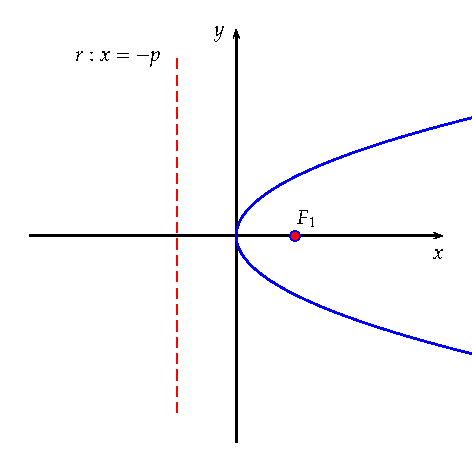
\includegraphics{parabola-foco-eixo-X-positivo.pdf}
  % \psset{ticksize=0pt}
  % \begin{pspicture*}(-4,-4)(4,4)
  %   \psaxes[labels=none]{->}(0,0)(-3.5,-3.5)(3.5,3.5)
  %   \rput{-90}(0,0){
  %     \psplot[algebraic,linecolor=blue
  %     ]{-2.0}{2.0}{x^2}
  %   }
  %   \psline[linestyle=dashed,linecolor=red](-1,-3)(-1,3)
  %   \rput(1.2,0.3){$F_1$}
  %   \psdot[linecolor=blue,fillcolor=red,dotstyle=o,dotsize=5pt](1,0)
  %   \rput(-2,3){$r: x = -p$}
  %   \rput(3.4,-0.3){$x$}
  %   \rput(-0.3,3.4){$y$}
  % \end{pspicture*}
\end{figure}

Agora, se a diretriz de $\mathcal{P}$ tem equa\c{c}\~ao $r: x = p$ e o foco \'e o ponto $F(-p,0)$, com $p > 0$, obtemos a equa\c{c}\~ao
\[
  y^2 = -4px.
\]
Neste caso, o gr\'afico da par\'abola \'e dado pela Figura \ref{FormageralParabola}.
\begin{figure}[!h]%par\'abola
  \centering
  \caption{Par\'abola $\mathcal{P}: y^2 = -4px$ e reta diretriz $r: x = p$, $p > 0$}
  \label{FormageralParabola}
  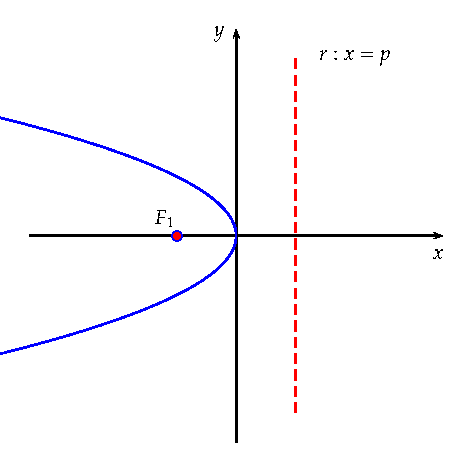
\includegraphics{parabola-foco-eixo-X-negativo.pdf}
  % \psset{ticksize=0pt}
  % \begin{pspicture*}(-4,-4)(4,4)
  %   \psaxes[labels=none]{->}(0,0)(-3.5,-3.5)(3.5,3.5)
  %   \rput{90}(0,0){
  %     \psplot[algebraic,linecolor=blue
  %     ]{-2.0}{2.0}{x^2}
  %   }
  %   \rput(-1.2,0.3){$F_1$}
  %   \psdot[linecolor=blue,fillcolor=red,dotstyle=o,dotsize=5pt](-1,0)
  %   \psline[linestyle=dashed,linecolor=red](1,-3)(1,3)
  %   \rput(2,3){$r: x = p$}
  %   \rput(3.4,-0.3){$x$}
  %   \rput(-0.3,3.4){$y$}
  % \end{pspicture*}
\end{figure}

Nos demais casos temos:
\begin{figure}[!h]%par\'abola
  \centering
  \caption{Par\'abola $\mathcal{P}: x^2 = -4py$ e reta diretriz $r: y = p$, $p > 0$}
  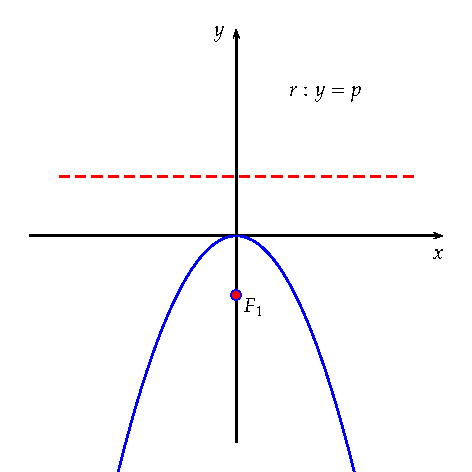
\includegraphics{parabola-foco-eixo-Y-negativo.pdf}
  % \psset{ticksize=0pt}
  % \begin{pspicture*}(-4,-4)(4,4)
  %   \psaxes[labels=none]{->}(0,0)(-3.5,-3.5)(3.5,3.5)
  %     \psplot[algebraic,linecolor=blue
  %     ]{-2.0}{2.0}{-x^2}
  %   \rput(0.3,-1.2){$F_1$}
  %   \psdot[linecolor=blue,fillcolor=red,dotstyle=o,dotsize=5pt](0,-1)
  %   \psline[linestyle=dashed,linecolor=red](-3,1)(3,1)
  %   \rput(1.5,2.4){$r: y = p$}
  %   \rput(3.4,-0.3){$x$}
  %   \rput(-0.3,3.4){$y$}
  % \end{pspicture*}
\end{figure}

\begin{figure}[!h]%par\'abola
  \centering
  \caption{Par\'abola $\mathcal{P}: x^2 = 4py$ e reta diretriz $r: y = -p$, $p > 0$}
  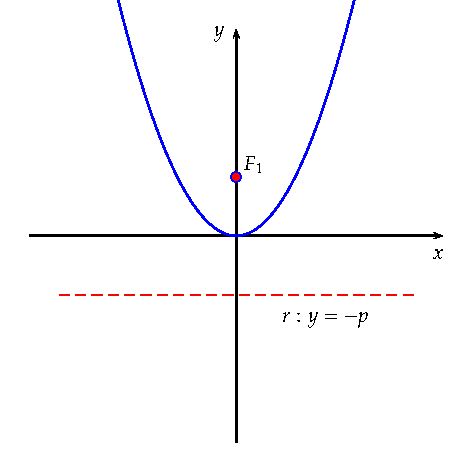
\includegraphics{parabola-foco-eixo-Y-positivo.pdf}
  % \psset{ticksize=0pt}
  % \begin{pspicture*}(-4,-4)(4,4)
  %   \psaxes[labels=none]{->}(0,0)(-3.5,-3.5)(3.5,3.5)
  %     \psplot[algebraic,linecolor=blue
  %     ]{-2.0}{2.0}{x^2}
  %   \rput(0.3,1.2){$F_1$}
  %   \psdot[linecolor=blue,fillcolor=red,dotstyle=o,dotsize=5pt](0,1)
  %   \psline[linestyle=dashed,linecolor=red](-3,-1)(3,-1)
  %   \rput(1.5,-1.4){$r: y = -p$}
  %   \rput(3.4,-0.3){$x$}
  %   \rput(-0.3,3.4){$y$}
  % \end{pspicture*}
\end{figure}

\begin{proposicao}
  As equa\c{c}\~oes $y^2 = qx$ e $x^2 = qy$ descrevem uma par\'abola se, e somente se, $q \ne 0$.
\end{proposicao}
% subsection parabolas (end)
% section conicas (end)

\section{Rota\c{c}\~ao e Transla\c{c}\~ao de Eixos} % (fold)
\label{sec:rotacao_e_translacao_de_eixos}


Para determinar a c\^onica representada pela equa\c{c}\~ao \eqref{equacaoconica} iremos utilizar transla\c{c}\~oes e rota\c{c}\~oes de eixos para simplificar sua equa\c{c}\~ao.

\subsection{Transla\c{c}\~ao de eixos} % (fold)
\label{sub:translacaoo_de_eixos}
Considere a seguinte c\^onica
\begin{equation}\label{conicaexemplo}
  x^2 + 2y^2 - 4x - 4y - 1 = 0.
\end{equation}
Podemos escrever
\begin{align*}
  &(x^2 - 4x + 4) - 4 + 2(y^2 - 2y + 1 - 1) - 1 = 0\\
  &(x - 2)^2 - 4 + 2(y - 1)^2 - 2 - 1 = 0\\
  &(x - 2)^2 + 2(y - 1)^2 = 7.
\end{align*}
Fazendo a mudan\c{c}a
\begin{align}
  x - 2 = x_1\label{mudancaX}\\
  y - 1 = y_1\label{mudancaY}
\end{align}
obtemos
\[
  \dfrac{x_1^2}{7} + \dfrac{y_1^2}{\dfrac{7}{2}}
\]
que representa uma elipse com focos no eixo $x_1$.

O efeito das equa\c{c}\~oes \eqref{mudancaX} e \eqref{mudancaY} foi o de mudar o centro da elipse de equa\c{c}\~ao \eqref{conicaexemplo} que estava no ponto $(2,1)$ no sistema original para o ponto $(0,0)$ considerando os eixos coordenados $x_1$ e $y_1$. 

Utilizando-se as equa\c{c}\~oes \eqref{mudancaX} e \eqref{mudancaY} podemos facilmente escrever as coordenadas de um ponto $P$ qualquer, tanto em rela\c{c}\~ao ao sistema de eixos coordenados $x$ e $y$, quanto ao sistema de eixos coordenados $x_1$ e $y_1$. Por exemplo, o ponto $P$ de coordenadas $P = (4,0)$, em rela\c{c}\~ao ao sistema $xy$, ter\'a coordenadas $(2,-1)$ em rela\c{c}\~ao ao sistema de eixos $x_1y_1$. As mudan\c{c}as introduzidas pelas equa\c{c}\~oes \eqref{mudancaX} e \eqref{mudancaY} s\~ao chamadas de \textbf{transla\c{c}\~oes de eixos}. De modo geral, se $(x,y)$ s\~ao as coordenadas de um ponto $P$ em rela\c{c}\~ao ao ponto $(0,0)$, ent\~ao as coordenadas de $P$ em rela\c{c}\~ao aos eixos $x_1$ e $y_1$, centrados no ponto $(a,b)$ s\~ao dadas por\index{Transla\c{c}\~ao de Eixos}
\begin{align}
  x_1 = x - a\label{mudancaXgeral}\\
  y_1 = y - b\label{mudancaYgeral}.
\end{align}

\begin{figure}[!h]
  \centering
  \caption{Transla\c{c}\~ao de eixos}
  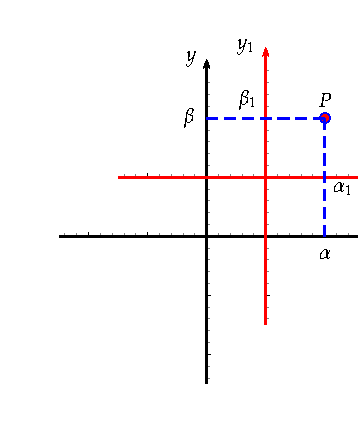
\includegraphics{translacao-eixos.pdf}
  % \begin{minipage}[b]{0.5\linewidth}
  %   \psset{ticksize=2pt}
  %   \begin{pspicture*}(-3.5,-3.5)(4,4)
  %     \psaxes[subticks=5,labels=none]{->}(0,0)(-2.5,-2.5)(3,3)[$x$,0][$y$,-180]
  %     \rput(2,-0.3){$\alpha$}
  %     \rput(-0.3,2){$\beta$}
  %     \psaxes[subticks=5,labels=none,linecolor=red]{->}(1,1)(-1.5,-1.5)(3.5,3.2)[$x_1$,0][$y_1$,-180]
  %     \rput(2.3,0.8){$\alpha_1$}
  %     \rput(0.7,2.3){$\beta_1$}
  %     \rput(2,2.3){$P$}
  %     \psdot[linecolor=blue,fillcolor=red,dotstyle=o,dotsize=5pt](2,2)
  %     \psline[linestyle=dashed,linecolor=blue](2,0)(2,2)
  %     \psline[linestyle=dashed,linecolor=blue](0,2)(2,2)
  %   \end{pspicture*}
  % \end{minipage}
\end{figure}
As mudan\c{c}as introduzidas pelas equa\c{c}\~oes \eqref{mudancaXgeral} e \eqref{mudancaYgeral} permitem remover os termos lineares da equa\c{c}\~ao \eqref{equacaoconica}.

\begin{exemplos}
  Identifique as c\^onicas:
  \begin{enumerate}
    \item $4x^2 - 8x + 9y^2 - 36y + 4 = 0$
    \begin{solucao}
      Completando quadrados
      \begin{align*}
        &4(x^2 - 2x + 1 - 1) + 9(y^2 - 4y + 4 - 4) + 4 = 0\\
        &4(x - 1)^2 + 9(y - 2)^2 = 36.
      \end{align*}
      Fazendo
      \begin{align*}
        x - 1 = x_1\\
        y - 2 = y_1
      \end{align*}
      obtemos
      \[
        \dfrac{x_1^2}{9} + \dfrac{y_1^2}{4} = 1
      \]
      que representa uma elipse com focos no eixo $x_1$. No novo sistema de coordenadas centrado no ponto os v\'ertices s\~ao
      \begin{align*}
        \overline{A_1}(-3,0),\quad \overline{A_2}(3,0)\\
        \overline{B_1}(0,-2),\quad \overline{B_2}(0,2).
      \end{align*}
      No sistema original os v\'ertices s\~ao
      \begin{align*}
        A_1(-2,2),\quad A_2(2,2)\\
        B_1(1,0),\quad B_2(1,4).
      \end{align*}
       \begin{figure}[!h]
        \centering
        \caption{Elipse $4x^2 - 8x + 9y^2 - 36y + 4 = 0$}
        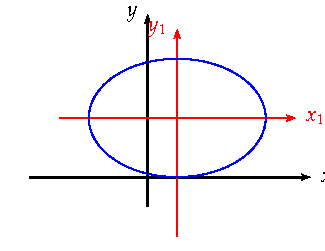
\includegraphics{elipse-eixos-tranladados.pdf}
        % \psset{unit=0.5cm}
        % \psset{ticksize=0pt}
        % \begin{pspicture*}(-5,-2.5)(6,6)
        %   \psaxes[labels=none]{->}(0,0)(-4,-1)(5.5,5.5)[$x$,0][$y$,-180]
        %   \psaxes[labels=none,linecolor=red]{->}(1,2)(-3,-2)(5,5)[$\color{red} x_1$,0][$\color{red} y_1$,-180]
        %   \psplotImp[algebraic,linecolor=blue,stepFactor=0.1,linewidth=0.5pt](-4,-1)(6,7){4*x^2 - 8*x + 9*y^2 - 36*y + 4}
        % \end{pspicture*}
      \end{figure}
    \end{solucao}
    \item $x^2 - 2y^2 - 6x - 8y - 1 = 0$
    \begin{solucao}
      Completando quadrados
      \begin{align*}
        &(x^2 - 6x + 9 - 9) - 2(y^2 + 4y + 4 - 4) - 1 = 0\\
        &(x - 3)^2 - 2(y + 2)^2 = 2.
      \end{align*}
      Fazendo
      \begin{align*}
        x - 3 = x_1\\
        y + 2 = y_1
      \end{align*}
      obtemos
      \[
        \dfrac{x_1^2}{2} - y_1^2 = 1
      \]
      que representa uma hip\'erbole com focos no eixo $x_1$. Suas ass{\'\i}ntotas s\~ao
      \[
        y_1 = \pm \dfrac{x_1}{\sqrt{2}}.
      \]
      Os v\'ertices s\~ao $\overline{A_1}(-\sqrt{2},0)$ e $\overline{A_2}(\sqrt{2},0)$.
      No sistema original suas ass{\'\i}ntotas s\~ao
      \begin{align*}
        y = \dfrac{x}{\sqrt{2}} - \left(\dfrac{3}{\sqrt{2}} + 2\right)\\
        y = -\dfrac{x}{\sqrt{2}} + \left(\dfrac{3}{\sqrt{2}} - 2\right).
      \end{align*}
      Os v\'ertices s\~ao $\overline{A_1}(-3 - \sqrt{2},0)$ e $\overline{A_2}(-3 + \sqrt{2},0)$.
       \begin{figure}[!h]
        \centering
        \caption{Hip\'erbole $x^2 - 2y^2 - 6x - 8y - 1 = 0$}
        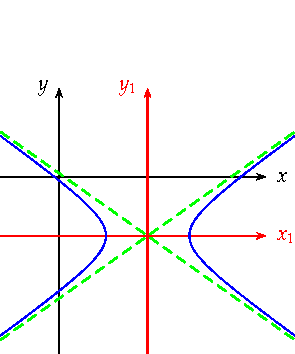
\includegraphics{hiperbole-eixos-tranladados.pdf}
        % \psset{unit=0.5cm}
        % \psset{ticksize=0pt}
        % \begin{pspicture*}(-2,-6)(8,6)
        %   \psaxes[labels=none]{->}(0,0)(-7,-7)(7,3)[$x$,0][$y$,-180]
        %   \psplot[algebraic,linestyle=dashed,linecolor=green]{-13}{13}{x/sqrt(2) - (3/sqrt(2) + 2)}
        %   \psplot[algebraic,linestyle=dashed,linecolor=green]{-13}{13}{-x/sqrt(2) + 3/sqrt(2) - 2}
        %   \psaxes[labels=none,linecolor=red]{->}(3,-2)(-7,-7)(7,3)[$\color{red} x_1$,0][$\color{red} y_1$,-180]
        %   \psplotImp[algebraic,linecolor=blue,stepFactor=0.1,linewidth=0.5pt](-4,-7)(10,7){(x-3)^2/2 - (y+2)^2  - 1}
        % \end{pspicture*}
      \end{figure}
    \end{solucao}
    \item $x^2 - y^2 - 2x - 6y = 8$
    \begin{solucao}
      Completando quadrados
      \begin{align*}
        &(x^2 - 2x + 1 - 1) - (y^2 + 6y + 9 - 9) - 1 = 0\\
        &(x - 1)^2 - (y + 3)^2 = 0\\
        &[(x - 1) - (y + 3)][(x - 1) + (y + 3)] = 0
      \end{align*}
      que representam as retas
      \begin{align*}
        r: x - y - 4 = 0\\
        s: x + y + 2 = 0
      \end{align*}
      que se interceptam no ponto $(1,-3)$.
    \end{solucao}
  \end{enumerate}
\end{exemplos}
% % subsection translacaoo_de_eixos (end)

\subsection{Rota\c{c}\~ao de eixos} % (fold)
\label{sub:rotacao_de_eixos}

Considere o sistema cartesiano com centro em $(0,0)$. Sejam $\vec{e_1} = (1,0)$ e $\vec{e_2} = (0,1)$. Para qualquer vetor $\vec{P} = (x,y)$ podemos escrever
\begin{align}\label{equacaoxy}
  \vec{P} = (x,y) = (x,0) + (0,y) = x(1,0) + y(0,1) = x\vec{e_1} + y\vec{e_2}.
\end{align}

\begin{figure}[!h]
  \centering
  \caption{Rota\c{c}\~ao de eixos: vetores $\vec{e_1}$ e $\vec{e_2}$}
  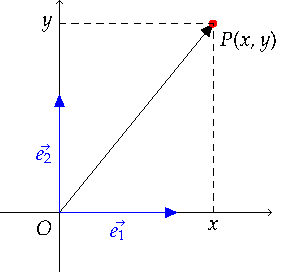
\includegraphics{rotacao-eixos-vetores-base.pdf}
  % \begin{tikzpicture}[scale=2]%vetor no plano
  %   \coordinate[label=below left:$O$] (A) at (0,0);
  %   \coordinate (W) at (1.3,1.6);
  %   %defini\c{c}\~ao das coordenadas dos eixos cartesianos
  %   \coordinate (F) at (-0.5,0);
  %   \coordinate (G) at (0,-0.5);
  %   \coordinate (X) at (1.8,0);
  %   \coordinate (Y) at (0,1.8);
  %   % Styles
  %   \tikzstyle{axes}=[]

  %   \begin{scope}[style=axes]%constr\'oi os eixos cartesianos
  %   \draw[->] (F) -- (X);
  %   \draw[->] (G) -- (Y);
  %   \end{scope}

  %   \draw[->,>=triangle 45] (A)--(W)
  %     node[below right]{$P(x, y)$};
  %     \draw [fill,color=red] (W) circle [radius=0.03];
  %   \draw[dashed,color=black] let \p1 = (W) in (\x1,0) -- (\x1,\y1)
  %     node[at start, below]{$x$};
  %   \draw[dashed,color=black] let \p1 = (W) in (0,\y1) -- (\x1,\y1)
  %     node[at start, left]{$y$};
  %   \draw[->,>=triangle 45,color=blue] (0,0) -- (1,0)
  %     node[midway, below]{$\vec{e_1}$};
  %     \draw[->,>=triangle 45,color=blue] (0,0) -- (0,1)
  %     node[midway, left]{$\vec{e_2}$};
  % \end{tikzpicture}
\end{figure}

Agora, efetuando-se uma rota\c{c}\~ao no sentido antihor\'ario nos eixos $x$ e $y$ de um \^angulo $\theta$, obtemos novos eixos coordenados $x_1$ e $y_1$. Tome vetores unit\'atios $\vec{u_1}$ e $\vec{u_1}$ nos eixos $x_1$ e $y_1$. Em rela\c{c}\~ao aos eixos originais podemos escrever
\begin{figure}[!h]
  \centering
  \caption{Rota\c{c}\~ao dos eixos por um \^angulo $\theta$}
  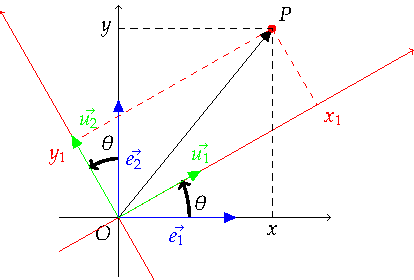
\includegraphics{rotacao-eixos.pdf}
  % \begin{tikzpicture}[scale=2]%vetor no plano
  %   \coordinate[label=below left:$O$] (A) at (0,0);
  %   \coordinate (W) at (1.3,1.6);
  %   %defini\c{c}\~ao das coordenadas dos eixos cartesianos
  %   \coordinate (F) at (-0.5,0);
  %   \coordinate (G) at (0,-0.5);
  %   \coordinate (X) at (1.8,0);
  %   \coordinate (Y) at (0,1.8);
  %   \coordinate (F1) at (-0.5,-0.285);%y=0,57x
  %   \coordinate (G1) at (0.3,-0.525);%y=-1,75x
  %   \coordinate (X1) at (2.5,1.42);%y=0,57x
  %   \coordinate (Y1) at (-1,1.75);%y=-1,75x
  %   % Styles
  %   \tikzstyle{axes}=[]

  %   \begin{scope}[style=axes]%constr\'oi os eixos cartesianos
  %     \draw[->] (F) -- (X);
  %     \draw[->] (G) -- (Y);
  %     \draw[->,color=red] (F1) -- (X1);
  %     \draw[->,color=red] (G1) -- (Y1);
  %   \end{scope}

  %   \draw [->,black,very thick](A) +(0:.6cm) arc (0:23:.8cm);
  %   \node at ($(A)+(10:7mm)$) {$\theta$};
  %   \draw [->,black,very thick](0,0.5) +(.4cm:0) arc (90:128:.4cm);
  %   \node at ($(0,0.5)+(125:1.6mm)$) {$\theta$};
  %   \draw[->,>=triangle 45] (A)--(W)
  %     node[at end,above right]{$P$};
  %   \draw [fill,color=red] (W) circle [radius=0.03];
  %   \draw[dashed,red] (W) -- ($(A)!(W)!(X1)$)
  %     node[at end,below right]{$x_1$};
  %   \draw[dashed,red] (W) -- ($(A)!(W)!(Y1)$)
  %     node[at end,below left]{$y_1$};
  %   \draw[dashed,color=black] let \p1 = (W) in (\x1,0) -- (\x1,\y1)
  %     node[at start, below]{$x$};
  %   \draw[dashed,color=black] let \p1 = (W) in (0,\y1) -- (\x1,\y1)
  %     node[at start, left]{$y$};
  %   \draw[->,>=triangle 45,color=blue] (0,0) -- (1,0)
  %     node[midway, below]{$\vec{e_1}$};
  %     \draw[->,>=triangle 45,color=blue] (0,0) -- (0,1)
  %     node[midway, right]{$\vec{e_2}$};
  %   \draw[->,>=triangle 45,color=green] (0,0) -- (0.7,0.399)%y=0,57x
  %     node[at end, above]{$\vec{u_1}$};
  %     \draw[->,>=triangle 45,color=green] (0,0) -- (-0.399,0.699)%y=-1,75x
  %     node[at end, above right]{$\vec{u_2}$};
  % \end{tikzpicture}
\end{figure}
\begin{align*}
  &\vec{u_1} = (\cos\theta,\sin\theta) = \cos\theta\vec{e_1} + \sin\theta\vec{e_2}\\
  &\vec{u_2} = (-\sin\theta,\cos\theta) = -\sin\theta\vec{e_1} + \cos\theta\vec{e_2}.
\end{align*}
Mas, os vetores $\vec{u_1}$ e $\vec{u_2}$ s\~ao unit\'arios e ortogonais, assim podemos escrever o vetor $\vec{P}$ como combina\c{c}\~ao de escalares nos eixos rotacionados, isto \'e,
\begin{equation}\label{equacaox1y1}
  \vec{P} = x_1\vec{u_1} + y_1\vec{u_2}.
\end{equation}

Da{\'\i} de \eqref{equacaoxy} e \eqref{equacaox1y1} obtemos
\[
  x\vec{e_1} + y\vec{e_2} = x_1\vec{u_1} + y_1\vec{u_2}
\]
e substituindo $\vec{u_1}$ e $\vec{u_2}$
\[
  x\vec{e_1} + y\vec{e_2} = (x_1\cos\theta - y_1\sin\theta)\vec{e_1} + (x_1\sin\theta + y_1\cos\theta)\vec{e_2}.
\]
Logo
\begin{align}
  &x = x_1\cos\theta - y_1\sin\theta\label{rotacaoX}\\
  &y = x_1\sin\theta + y_1\cos\theta\label{rotacaoY}
\end{align}
e ent\~ao isolando $x_1$ e $y_1$
\begin{align*}
  &x_1 = x\cos\theta + y\sin\theta\\
  &y_1 = -x\sin\theta + y\cos\theta.
\end{align*}
Portanto para eliminar o termo $xy$ da equa\c{c}\~ao $g(x,y) = 0$, substitu{\'\i}mos \eqref{rotacaoX} e \eqref{rotacaoY} em $g(x,y) = 0$ e determinanos o \^angulo $\theta$ que elimina o termo $xy$.

\begin{exemplos}
  Seja $P$ o ponto $P(6,4)$. Efetuando-se uma rota\c{c}\~ao de um \^angulo de $\theta = \pi/3$ radianos nos eixos, as coordenadas de $P$ em rela\c{c}\~ao aos novos eixos s\~ao
    \begin{align*}
      x_1 = 6\cos(\pi/3) + 4\sin(\pi/3) = 3 + 2\sqrt{3}\\
      y_1 = -6\sin(\pi/3) + 4\cos(\pi/3) = 2 - 3\sqrt{3}.
    \end{align*}
    Da{\'\i} no novo sistema $P(3 + 2\sqrt{3}, 2 - 3\sqrt{3})$.
\end{exemplos}

\begin{exemplos}
  Identifique as c\^onicas:
  \begin{enumerate}
    \item $3x^2 + 3y^2 - 10xy + 12\sqrt{2}x - 4\sqrt{2}y + 32 = 0$
    \begin{solucao}
      Fazendo as mudan\c{c}as
      \begin{align}
        x = x_1\cos\theta - y_1\sin\theta\\
        x = x_1\sin\theta + y_1\cos\theta
      \end{align}
      temos
      \begin{align*}
        &3(x_1\cos\theta - y_1\sin\theta)^2 + 3(x_1\sin\theta + y_1\cos\theta)^2\\ &- 10(x_1\cos\theta - y_1\sin\theta)(x_1\sin\theta + y_1\cos\theta)\\ & + 12\sqrt{2}(x_1\cos\theta - y_1\sin\theta) - 4\sqrt{2}(x_1\sin\theta + y_1\cos\theta)\\ &= (3\cos^2\theta + 3\sin^2\theta - 10\sin\theta\cos\theta)x_1^2 \\ &+ (3\sin^2\theta + 3\cos^2\theta + 10\sin\theta\cos\theta)y_1^2 \\ &+ (6\sin\theta\cos\theta - 10\cos^2\theta + 10\sin^2\theta - 6\sin\theta\cos\theta)x_1y_1 \\ &+ (12\sqrt{2}\cos\theta - 4\sqrt{2}\sin\theta)x_1 + (-12\sqrt{2}\sin\theta - 4\sqrt{2}\cos\theta)y_1 + 32 = 0.
      \end{align*}
      Assim $\theta$ deve ser tal que
      \[
        -10\cos^2\theta + 10\sin^2\theta = 0,
      \]
      isto \'e, $\theta = \pi/4$. Substituindo esse valor de $\theta$ na equa\c{c}\~ao anterior e simplificando obtemos
      \[
        x_1^2 - 4y_1^2 - 4x_1 + 8y_1 - 16 = 0.
      \]
      Nessa nova equa\c{c}\~ao podemos completar quadrados
      \begin{align*}
        &(x_1^2 - 4x_1 + 4) - 4 - 4(y_1^2 - 2y_1 + 1 - 1) - 16 = 0\\
        &(x_1 - 2)^2 - 4(y_1 - 1)^2 = 16.
      \end{align*}
      Fazendo
      \begin{align*}
        x_2 = x_1 - 2\\
        y_2 = y_1 - 1
      \end{align*}
      encontramos
      \[
        \dfrac{x_2^2}{16} - \dfrac{y_2^2}{4} = 1
      \]
      que \'e uma hip\'erbole de v\'ertices no eixo $x_2$.
      \begin{figure}[!h]
        \centering
        \caption{Hip\'erbole $3x^2 +3y^2 - 10xy + 12\sqrt{2}x - 4\sqrt{2}y + 32 = 0$}
        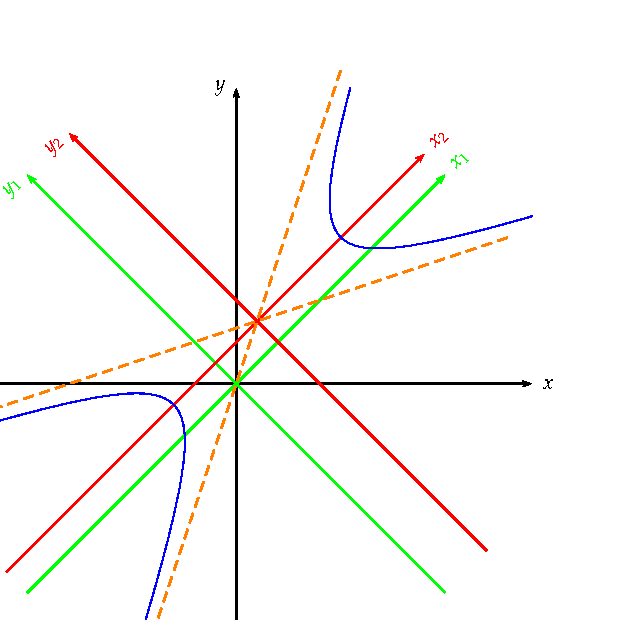
\includegraphics{hiperbole-rotacionada-transladada.pdf}
        % \psset{unit=0.5cm}
        % \psset{ticksize=0pt}
        % \begin{pspicture*}(-8,-8)(13,13)
        %   \psaxes[labels=none]{->}(0,0)(-10,-10)(10,10)[$x$,0][$y$,-180]
        %   \rput{45}(0,0){
        %     \psaxes[labels=none,linecolor=green]{->}(0,0)(-10,-10)(10,10)[$\color{green} x_1$,0][$\color{green} y_1$,-180]  
        %   }
        %   \rput{45}(0,0){
        %     \psaxes[labels=none,linecolor=red]{->}(2,1)(-10,-10)(10,10)[$\color{red} x_2$,0][$\color{red} y_2$,-180]
        %     \psplot[algebraic,linestyle=dashed,linecolor=orange]{-10}{10}{x/2}
        %     \psplot[algebraic,linestyle=dashed,linecolor=orange]{-10}{10}{-x/2+2}
        %   }
        %   \psplotImp[algebraic,linecolor=blue,stepFactor=0.1,linewidth=0.5pt](-10,-10)(10,10){3*x^2 + 3*y^2 - 10*x*y + 12*sqrt(2)*x - 4*sqrt(2)*y + 32}
        % \end{pspicture*}
      \end{figure}
    \end{solucao}
    \item $52x^2 - 72xy + 73y^2 - 400 = 0$
    \begin{solucao}
      Fazendo as mudan\c{c}as
      \begin{align}
        x = x_1\cos\theta - y_1\sin\theta\\
        x = x_1\sin\theta + y_1\cos\theta
      \end{align}
      temos
      \begin{align}\label{conicaelipse}
        &52(x_1\cos\theta - y_1\sin\theta)^2 + 73(x_1\sin\theta + y_1\cos\theta)^2\nonumber \\ &- 72(x_1\cos\theta - y_1\sin\theta)(x_1\sin\theta + y_1\cos\theta) - 400 = 0\nonumber\\ &(52\cos^2\theta - 72\sin\theta\cos\theta + 73\sin^2\theta)x_1^2 + (52\sin^2\theta + 72\sin\theta\cos\theta + 73\cos^2\theta)y_1^2 \nonumber\\&+ (-104\sin\theta\cos\theta + 72\sin^2\theta - 72\cos^2\theta + 146\sin\theta\cos\theta)x_1y_1 - 400 = 0
      \end{align}
      Assim devemos ter
      \begin{align*}
        &-104\sin\theta\cos\theta + 72\sin^2\theta - 72\cos^2\theta + 146\sin\theta\cos\theta = 0\\
        &42\sin\theta\cos\theta + 72(\sin^2\theta - \cos^2\theta) = 0\\
        &21\sin(2\theta) - 72\cos(2\theta) = 0\\
        &\tan(2\theta) = \dfrac{24}{7}.
      \end{align*}
      Agora
      \[
        \cos(2\theta) = \dfrac{1}{\sqrt{1 + \tan^2(2\theta)}}
      \]
      e usando as equa\c{c}\~oes $\cos^2\theta = (1/2)(1 + \cos(2\theta))$ e $\sin^2\theta = (1/2)(1 - \cos(2\theta))$ obtemos
      \[
        \cos\theta = \dfrac{4}{5} \quad \mbox{e}\quad \sin\theta = \dfrac{3}{5}.
      \]
      Substituindo na equa\c{c}\~ao \eqref{conicaelipse} obtemos
      \begin{align*}
        &\left(52\dfrac{16}{25} - 72\dfrac{12}{25} + 73\dfrac{9}{25}\right)x_1^2 + \left(52\dfrac{9}{25} + 72\dfrac{12}{25} + 73\dfrac{16}{25}\right)y_1^2 - 400 = 0\\
        &25x_1^2 + 100y_1^2 = 400\\
        &\dfrac{x_1^2}{16} + \dfrac{y_1^2}{4} = 1
      \end{align*}
      que representa uma elipse com focos no eixo $x_1$.
      \begin{figure}[!h]
        \centering
        \caption{Elipse $52x^2 - 72xy + 73y^2 - 400 = 0$}
        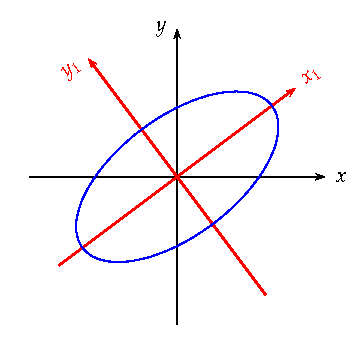
\includegraphics{elipse-rotacionada.pdf}
        % \psset{unit=0.5cm}
        % \psset{ticksize=0pt}
        % \begin{pspicture*}(-6,-6)(6,6)
        %   \psaxes[labels=none]{->}(0,0)(-5,-5)(5,5)[$x$,0][$y$,-180]
        %   \rput{36.87}(0,0){
        %     \psaxes[labels=none,linecolor=red]{->}(0,0)(-5,-5)(5,5)[$\color{red} x_1$,0][$\color{red} y_1$,-180]  
        %   }
        %   \psplotImp[algebraic,linecolor=blue,stepFactor=0.1,linewidth=0.5pt](-10,-10)(10,10){52*x^2 - 72*x*y + 73*y^2 - 400}
        % \end{pspicture*}
      \end{figure}
    \end{solucao}
    \item $x^2 - 2xy + y^2 - 2x - 2y + 1 = 0$
    \begin{solucao}
      Fazendo as mudan\c{c}as
      \begin{align}
        x = x_1\cos\theta - y_1\sin\theta\\
        x = x_1\sin\theta + y_1\cos\theta
      \end{align}
      temos
      \begin{align}\label{conicaparabola}
        &(x_1\cos\theta - y_1\sin\theta)^2 - 2(x_1\cos\theta - y_1\sin\theta)(x_1\sin\theta + y_1\cos\theta)\nonumber \\&+ (x_1\sin\theta + y_1\cos\theta)^2 - 2(x_1\cos\theta - y_1\sin\theta) - 2(x_1\sin\theta + y_1\cos\theta) + 1 = 0\nonumber\\
        &(\cos^2\theta - 2\sin\theta\cos\theta + \sin^2\theta)x_1^2 + (\sin^2\theta + 2\sin\theta\cos\theta + \cos^2\theta)y_1^2\nonumber\\ &+ (-2\sin\theta\cos\theta - 2\cos^2\theta + 2\sin^2\theta + 2\sin\theta\cos\theta)x_1y_1\nonumber\\ &+ (-2\cos\theta - 2\sin\theta)x_1 + (2\sin\theta - 2\cos\theta)y_1 + 1 = 0.
      \end{align}
      Assim devemos ter
      \[
        -2\cos^2\theta + 2\sin^2\theta = 0,
      \]
      isto \'e, $\theta = \pi/4$. Substituindo em \eqref{conicaparabola} obtemos a equa\c{c}\~ao
      \[
        y_1^2 = \sqrt{2}\left(x_1 - \dfrac{1}{2\sqrt{2}}\right).
      \]
      Fazendo
      \begin{align*}
        x_1 - \dfrac{1}{2\sqrt{2}} = x_2\\
        y_1 = y_2
      \end{align*}
      encontramos
      \[
        y_2^2 = \sqrt{2}x_2
      \]
      que representa uma par\'abola com foco no eixo $x_2$ e reta diretriz $x_2 = -\sqrt{2}/4$.
      \begin{figure}[!h]
        \centering
        \caption{Par\'abola $x^2 - 2xy + y^2 - 2x - 2y + 1 = 0$}
        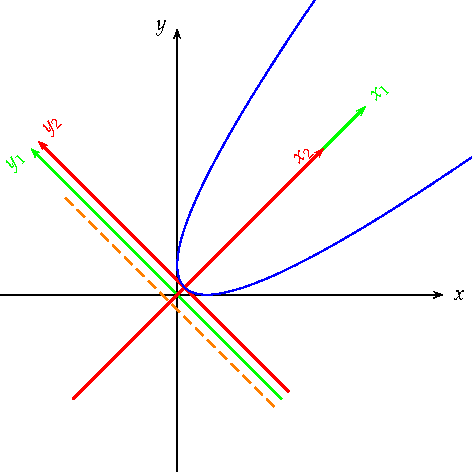
\includegraphics{parabola-rotacionada-transladada.pdf}
        % \psset{unit=0.5cm}
        % \psset{ticksize=0pt}
        % \begin{pspicture*}(-6,-6)(10,10)
        %   \psaxes[labels=none]{->}(0,0)(-6,-6)(9,9)[$x$,0][$y$,-180]
        %   \rput{45}(0,0){
        %     \psaxes[labels=none,linecolor=green]{->}(0,0)(-5,-5)(9,7)[$\color{green} x_1$,0][$\color{green} y_1$,-180]  
        %   }
        %   \rput{45}(0,0){
        %     \psaxes[labels=none,linecolor=red]{->}(0.3535,0)(-5,-5)(7,7)[$\color{red} x_2$,150][$\color{red} y_2$,0]
        %     \psline[linestyle=dashed,linecolor=orange](-0.3535,-5)(-0.3535,5)
        %   }
        %   \psplotImp[algebraic,linecolor=blue,stepFactor=0.1,linewidth=0.5pt](-10,-10)(10,10){x^2 - 2*x*y + y^2 - 2*x - 2*y + 1}
        % \end{pspicture*}
      \end{figure}
    \end{solucao}
  \end{enumerate}
\end{exemplos}

% subsection rotacao_de_eixos (end)

% section rotacao_e_translacao_de_eixos (end)

% \section{Se\c{c}\~oes C\^onicas} % (fold)
% \label{sec:secoes_conicas}
% \missingfigure{Figuras de se\c{c}\~oes c\^onicas}
% section secoes_conicas (end)

% chapter circunferencias_e_conicas (end)